%%%%%%%%%%%%%%%%%%%%%%%%%%%%%%%%%%%%%%%%%%%%%%%%%%%%%%%%%%%%%%%%%%%%%%%%%%%%%%%
% Neuroimage-like layout
% Neuroimage-like layout
%\documentclass[12pt,3p,review]{elsarticle}
%\documentclass[12pt,3p,review,number]{elsarticle}
\documentclass[12pt,5p]{elsarticle}
%\documentclass[5p]{elsarticle}
% For kindle
%\documentclass[1p,12pt]{elsarticle}
%\usepackage{geometry}
%\geometry{a6paper,hmargin={.2cm,.2cm},vmargin={1cm,1cm}}
% End kindle
\usepackage{amsmath,amsfonts,amssymb}
\usepackage{bm}
\usepackage{algorithm}
\usepackage{algorithmic}
\usepackage{url}
\usepackage[breaklinks=true,letterpaper=true,colorlinks,bookmarks=false]{hyperref}
\usepackage[table]{xcolor}
\usepackage[pagewise]{lineno}
\usepackage{varwidth}

\newcommand\MyCBox[1]{%
  \colorbox{yellow!60}{\begin{varwidth}{\dimexpr\linewidth-2\fboxsep}#1\end{varwidth}}}


\biboptions{sort}

\definecolor{deep_blue}{rgb}{0,.2,.5}
\definecolor{dark_blue}{rgb}{0,.15,.5}

\hypersetup{pdftex,  % needed for pdflatex
  breaklinks=true,  % so long urls are correctly broken across lines
  colorlinks=true,
  linkcolor=dark_blue,
  citecolor=deep_blue,
}

% Float parameters, for more full pages.
\renewcommand{\topfraction}{0.9}        % max fraction of floats at top
\renewcommand{\bottomfraction}{0.8}     % max fraction of floats at bottom
\renewcommand{\textfraction}{0.07}      % allow minimal text w. figs
%   Parameters for FLOAT pages (not text pages):
\renewcommand{\floatpagefraction}{0.6}  % require fuller float pages
%    % N.B.: floatpagefraction MUST be less than topfraction !!


\def\B#1{\mathbf{#1}}
%\def\B#1{\bm{#1}}
\def\trans{^\mathsf{T}}
% A compact fraction
\def\slantfrac#1#2{\kern.1em^{#1}\kern-.1em/\kern-.1em_{#2}}

%%%%%%%%%%%%%%%%%%%%%%%%%%%%%%%%%%%%%%%%%%%%%%%%%%%%%%%%%%%%%%%%%%%%%%%%%%%%%%
% For the final version: to output PDF figures from latex
\newif\iffinal
\finaltrue
%\finalfalse
\iffinal\else
\usepackage[tightpage,active]{preview}
\fi

%%%%%%%%%%%%%%%%%%%%%%%%%%%%%%%%%%%%%%%%%%%%%%%%%%%%%%%%%%%%%%%%%%%%%%%%%%%%%%
% Modification tracking
\usepackage{xcolor}
\usepackage[normalem]{ulem}
\colorlet{markercolor}{purple!50!black}
\colorlet{cc_commentcolor}{blue!20!black!30!green}
\newcommand{\ADDED}[1]{\textcolor{markercolor}{\uline{#1}}}
\newcommand{\DELETED}[1]{\textcolor{red}{\sout{#1}}}
\newcommand{\COMMENTCC}[1]{\MyCBox{\textcolor{cc_commentcolor}{\textbf{Cameron:
#1}}}}

% For highlighting changes for reviewer
\usepackage{MnSymbol}
\def\marker{%
    \vadjust{{%
	\llap{\smash{%
	    \color{purple}%
	    \scalebox{1.8}{$\filledmedtriangleright$}}\;}%
    }}\hspace*{-.1ex}%
}%
\def\hl#1{\textcolor{markercolor}{%
   \protect\marker%
  #1%
}}%



%%%%%%%%%%%%%%%%%%%%%%%%%%%%%%%%%%%%%%%%%%%%%%%%%%%%%%%%%%%%%%%%%%%%%%%%%%%%%%%%
\begin{document}

% Show line numbers
%\linenumbers
%\linenumbersep 3pt\relax
%\renewcommand\linenumberfont{\normalfont\tiny\sffamily\color{black!50}}
%\renewcommand\linenumberfont{\normalfont\color{dark_blue}}



\title{Bibliometric Analysis of Resting State fMRI Literature}

\author[cmi]{Matthew K. Doherty}
\author[cmi]{Ayesha Anwar}
\author[cmi]{Sam Barberie}
\author[cmi]{Caitlin Hinz}
\author[cmi]{Michelle Kaplan}
\author[cmi]{Anna Rachlin}
\author[cmi,nki]{Michael P. Milham}
\author[vtcri,vtbme]{Stephen M. LaConte}
\author[cmi,nki]{R. Cameron Craddock\corref{corresponding}}

\cortext[corresponding]{Corresponding author: cameron.craddock@childmind.org }

\address[cmi]{Child Mind Institute, New York, New York}
\address[nki]{Nathan Kline Institute for Psychiatric Research, 
    Orangeburg, New York}
\address[vtcri]{Virginia Tech Carilion Research Institute, Roanoke, Virginia}
\address[vtbme]{School of Biomedical Engineering and Sciences, Virginia Tech,
Blacksburg, Virginia}

\begin{abstract}
    Some cool stuff about why the Child Mind Librarian is so freaking cool ...
    and why we care, and other things of relative importance.
\end{abstract}

\begin{keyword}
    Functional connectivity, connectome, group study, effective
    connectivity, fMRI, resting-state
\end{keyword}

\maketitle
%%%%%%%%%%%%%%%%%%%%%%%%%%%%%%%%%%%%%%%%%%%%%%%%%%%%%%%%%%%%%%%%%%%%%%%%%%%%%%%%


\sloppy % Fed up with messed-up line breaks
%%%%%%%%%%%%%%%%%%%%%%%%%%%%%%%%%%%%%%%%%%%%%%%%%%%%%%%%%%%%%%%%%%%%%%%%%%%%%%%

\section{Introduction}

Since its initial observation in 1995 \cite{Biswal1995}, resting state
functional magnetic resonance imaging (R-fMRI) has exploded in popularity
as a technique for studying the brain’s functional architecture. Although
initially plagued by controversies related to the physiological
underpinnings and unconstrained nature of R-fMRI
\cite{Lund2001,Morcom2007}, it has persevered to become a standard
assessment in basic, clinical and cognitive neurosciences
\cite{Fox2010,Kelly2012}.  The result is a burgeoning literature dedicated
to R-fMRI that is quickly becoming unwieldy for researchers to navigate.
The Child Mind Institute (CMI) Librarian initiative addresses this
challenge by providing a hand-curated reference library of R-fMRI
literature (http://www.mendeley.com/profiles/cmi-librarian). This library
consists of 1,721 publications (as of December 24, 2012) and requisite
metadata to facilitate the systematic review of its contents. We
inaugurate the availability of this open resource by performing a
bibliometric analysis to assess the current state of R-fMRI literature.

Bibliometrics involves the application of mathematics and statistical
methods to a body of literature to illuminate its course of development
and measure its impact \cite{Pritchard1969}. Although primarily concerned
with analyzing citations to estimate the impact of researchers and
particular papers within the field, bibliometrics can also identify common
themes within in the literature.  Bibliometric analyses differ from more
standard literature reviews in that they are largely automated and may
overlook or misinterpret details of individual publications that would be
apparent to a human reader. On the other hand, bibliometric analyses are
data-driven and can be more comprehensive, using a larger fraction of the
corpus to support its conclusions. The quality of the analyses is
determined by the quality of the literature database used for the
analysis. The CMI Librarian resting state literature database is ideal for
automated data mining because it has been hand-vetted to remove irrelevant
publications, and to provide basic keywords to inform the analysis.

This automated statistical analysis of R-fMRI literature incorporated
information from the CMI librarian database, PubMed (http://pubmed.gov),
and the full text of the publications. Information across these resources
was combined to gain insight into publication growth, venues and patterns.
Citation analyses were performed to identify publications and researchers
with the greatest impact, as well as to identify working groups of
researchers who tend to co-publish. Key word analyses were performed to
identify experimental methods, cognitive domains, clinical disorders, and
brain regions most commonly discussed in the literature. Together the
results from these analyses narrate the history of R-fMRI.

\section{Methods}

\subsection{CMI Librarian}

The CMI Librarian initiative has constructed a comprehensive database of
R-fMRI publications that is maintained in Mendeley (Mendeley, Inc., New
York, NY). The database is updated monthly using PubMed-based searches
that are run in Sente (Third Street Software, Inc., Denver, CO) with the
following query: \texttt{``resting state fMRI'' OR ``intrinsic functional
connectivity'' OR ``rest AND functional connectivity'' OR ``fmri AND
default mode network''}.  Abstracts corresponding to publications returned
from the search are hand vetted by CMI Librarian staff to exclude papers
that are duplicates, do not have an English language abstract, or are not
explicitly related to fMRI and resting state. Based on the content of the
abstracts, the articles are then assigned tags based on their topic areas.
Articles are marked as \emph{clinical} if they deal with a clinical
population of any kind, and are additionally tagged with the specific
disorder/population. The \emph{basic neuroscience} tag is applied to
papers that focus on non-clinical populations and are additionally
categorized as \emph{brain and behavior}, \emph{functional anatomy}, or
\emph{multimodal}. The latter refers to papers that integrate fMRI with an
additional imaging modality. There are additional tags for papers that
incorporate genetics (\emph{genetics}) and those that include animal
research (\emph{animal models}). Journal articles that are mainly focused
on a particular analytical or imaging technique are classified with the
\emph{methodology} tag.  Finally there are tags for reviews and
meta-analyses (\emph{review/meta-analysis}) and papers that use data from
the 1000 Functional Connectomes and International Neuroimaging
Data-sharing Initiative (\emph{1000 Functional Connectomes}). 

\subsection{Publication Trends}
Publication rates, venues, subject areas, and open access policies were
measured and analyzed using metadata found in the CMI Library and
complementary PubMed queries. The growth rates of literature volume over
time were found for R-fMRI and compared to that for all of fMRI - the
mother discipline of R-fMRI. First, the CMI Librarian was aggregated by
year to find each year’s publication count. Then, the following query was
used on PubMed to find the number of articles in all of fMRI per year:
\texttt{(``fMRI'' or ``functional magnetic resonance imaging'') and
(``YEAR''[Publication Date])}.  The cumulative sums were then calculated
to find the total literature volume over time.

Growth rates were modeled with exponential functions. An exponential
growth rate indicates that the literature’s growth rate
$\slantfrac{dV}{dt}$ is proportional to its volume ($V$),
$\slantfrac{dV}{dt} \propto V$.  To model publication growth, piecewise
exponential functions of the form $V(t)=V_0 e^{Rt}$ were fitted over the
intervals Janurary 1, 1994 - December 31, 2005 and Janurary 1, 2006 -
December 31, 2012 for both R-fMRI and fMRI. The year 1994 was chosen as
the first point because growth is subexponential before this period.
Between 1994 and 2012, growth is super-exponential if fitted over the full
period; so two piecewise curves were fitted. The break point at 2006 was
chosen by minimizing model error over the full period. 

Several additional publication trend statistics were computed from CMI
Librarian and PubMed metadata. Counts of publications by journal were
found directly from CMI Librarian data. Clinical applications were
aggregated from the library’s hand-curated tag information. Open access
rates for R-fMRI and all of fMRI were found from PubMed. 

Using address information from the CMI Librarian, a density-equalizing
map, or cartogram, was generated on the publications’ correspondence
addresses with the ScapeToad (http://scapetoad.choros.ch) implementation
of the Gastner/Newman diffusion-based algorithm \cite{Gastner2004}.  The
goal of the cartogram, and the Gastner/Newman algorithm in particular, is
to plot a geographical map such that the density of the publications by
country is constant per unit area, and the boundaries of each country are
still recognizable.

\subsection{Term Frequency Analysis}
A bag of words model was used to learn about the field’s experimental
methods and areas of focus. A bag of words model assumes that all of the
words in a corpus are statistically independent, regardless of whether
they appear in the same sentence or publication.  Under this model, a
term’s significance can be measured simply by counting its occurrences.
\COMMENTCC{Should we reference a text mining review here?}

Terms of interest were derived from n-grams (a phrase consisting of $n$
words) from neuroimaging methods, cognitive ontology \cite{Poldrack2011},
and the PubBrain lexicon (http://www.pubbrain.org). N-grams from cognitive
ontology and the PubBrain lexicon were found from their respective online
sources. A domain expert (RCC) manually generated the list of terms for
neuroimaging methods. The final sets of n-grams were found by iteratively
testing a candidate set, then combining synonyms and compound terms to
form a new candidate set.

For each term, conditional term frequency (conditional-$t\!f$) was
computed as the median ratio of term count to total word count in each
publication that contained the term of interest. Document frequency
($d\!f$) for each term was computed as the number of documents containing
the term. Terms with high $d\!f$ are popular across the corpus, while
terms with high conditional-$t\!f$ occur often in the documents in which
they appear.  

\subsection{Prevalence Of Methods} 
A Na\"ive Bayes model was used to determine the prevalence of various
analysis methods in the literature. \COMMENTCC{Include a citation for
this?} In particular, this model was used to discriminate papers that used
seed-based correlation, ICA, clustering, graph theory, and machine
learning methods. First, a small training set of 10 publications was
manually created.  From this training set, important features were derived
by finding tokens and n-grams with high values of the $\chi^2$ statistic,
which is used as a proxy for information gain \cite{Quinlan86}. A term
frequency matrix was then constructed, relating each publication to the
frequency of each term contained in the publication.  Logarithmic term
frequencies ($\log{t\!f}$) were used to prevent a single term from
dominating the model.  Each publication’s vector was normalized to unit
length to mitigate the effect of publications that contain too many or too
few terms. This term frequency matrix was used to train a Na\"ive Bayes
model.  Finally, 213 additional publications were classified by hand and
used to test the classification accuracy of the model.

\subsection{Citation Analysis}
Publications and the citations that link them were modeled as a directed
graph to characterize their relationships and ``small world'' nature
\cite{Watts1998}.  A directed graph is a general framework used to
represent relationships between nodes (publications) using edges
(citations), which each point from one node to another.

First, PDF files corresponding to the titles in the CMI Librarian were
systematically downloaded. A fuzzy search for every publication title in
every file was performed using the SequenceMatcher method of Pythons
difflib library (http://docs.python.org/2/library/difflib.html). This
fuzzy search first cleaned the binary file with regular expressions to
remove junk patterns and normalize whitespace. The longest identical match
of the publication title was compared to this match and its context to the
true publication title by finding the match ratio (measure of similarity
between strings). Of 20,541 total matches with ratio greater than or equal
to 0.8, 16,425 (80\%) had a ratio of 1.0—i.e., they were exact matches—and
17,983 (88\%) had a ratio at least 0.9. The cutoff for true matches was
set to 0.9, resulting in 17,983 citations. 

Using the citations found by the fuzzy search, a graph was constructed of
the CMI Librarian publications (nodes) and the citations between them
(edges). From this graph, the most central nodes were found using the
pagerank implementation in NetworkX \cite{Hagberg2008}. Pagerank, a
variant of eigenvector centrality, aims to find the steady state
probability of a random walk reaching each node \cite{Page1999}. These
solutions are given by the equation:

\begin{equation} P\!r(p_i)=\frac{1-d}{N} + d\!\sum_{p_j \in
M(p_i)}\frac{P\!r(p_i)}{L(p_j)} \end{equation}

\noindent where $N$ is number of nodes, $d$ is the probability of
continuing the random walk, $M(p)$ is the set of pages that link to node
$p$, and $L(p)$ is the number of outbound edges from $p$. The solutions,
$P\!r(p_i)$, are the dominant eigenvector of a modified adjacency matrix,
and can be found with the power method.

Finally, a jackknife procedure \cite{Quenouille1956} was performed to
reduce the variance of the Pageranks and to quantify their sensitivity to
choices of fuzzy-search parameters. For each of over 1,000 replicates,
20\% of the edges were randomly deleted, and Pagerank was calculated.  The
Pagerank mean and standard error over the jackknifes were reported, which
is an overestimate of the true procedure error.  Additionally, the graph's
mean shortest path length and mean clustering coefficient was calculated
in a seperate analysis.

\subsection{Graph Analysis of Co-authorships}
Collaborative relationships between authors of R-fMRI literature can be
characterized by co-authorships. A graph was constructed from the CMI
Librarian data in which each node corresponds to an author and edges
represent co-authorships, weighted by the number of papers that the two
authors appear on.  From this graph, we calculated average path length,
clustering coefficient, Pagerank centrality, and the quantity of disjoint
sets. Additionally, we tested for graph robustness by repeatedly removing
authors and publications and measuring graph connectivity.

\subsection{Working Groups}
We defined working groups as sets of researchers who frequently publish
together and, once found, the publication patterns of these groups were
examined. In order to find these groups, a greedy community-detection
algorithm was developed that uses the intersection of researchers’
publication sets to measure their similarity.

\COMMENTCC{ALGORITHM GOES HERE}

The procedure for identifying author working groups begins by repeatedly
seeding a new working group with the author with the most publications
(lines 2-3).  Authors are searched to find the author with the most
co-authored publications with the working group (line 6). If this author
has more than 10 publications, and is a co-author on at least 30\% of the
publications authored by the members of the working group (line 7), then
the author is added to the working group (line 6). Otherwise, the working
group is closed and considered for inclusion in the results. If the sum of
all papers in common across the candidate working group is greater than
50, and the working group has less than 20\% of authors in common with any
other working group (line 8), then it is included in the results (line 9).

\section{Results}

\subsection{Publication Trends}
Growth of R-fMRI literature was fitted by piecewise exponential functions
with 32\% growth between January 1,1994 and December 31, 2005 and 47\%
between January 1, 2006 and December 31, 2012. In comparison, growth of
fMRI literature was found to be 26\% and 17\% during the same time
periods. Fig.  \ref{fig:overallgrowth} shows the growth of each
literature, and represents a total of 28,434 fMRI publications and 1,721
R-fMRI publications. Additionally, 39\% of R-fMRI publications were
determined to be open access, compared to 31\% in all of fMRI.

%{{{------ Figure 1 -----}}}
\begin{figure}
  \begin{center}
    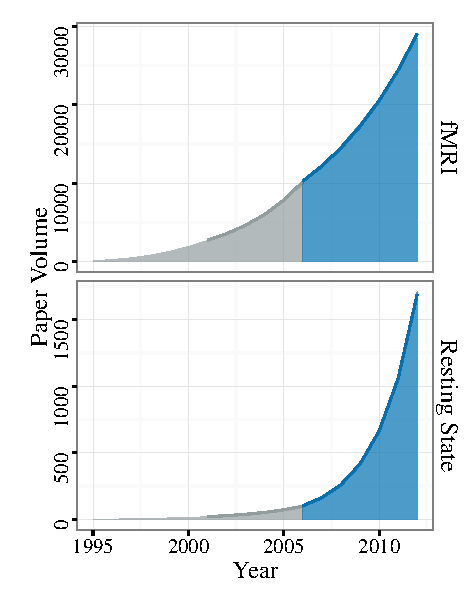
\includegraphics[]{figures/overall_growth}%
    %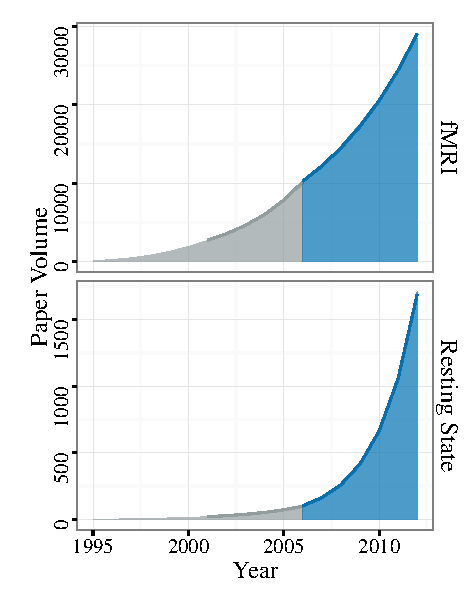
\includegraphics[width=\linewidth]{figures/overall_growth}%
    %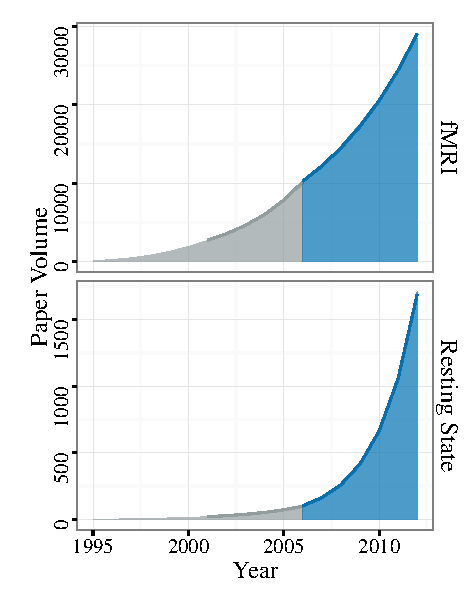
\includegraphics[width=.5\linewidth]{figures/overall_growth}%
    \caption{The growth of resting state and fMRI literature.
        \label{fig:overallgrowth}
    }
  \end{center}
\end{figure}


The top 20 publication outlets for R-fMRI publications accounted for 59\%
(1017) of the CMI R-fMRI library as shown in Fig. \ref{fig:journal_dist}.
This list is dominated by three neuroimaging journals (NeuroImage, Human
Brain Mapping, Brain Connectivity), which accounted for approximately 26\%
of the R-fMRI publications. The top 20 also include nine general
neuroscience, two general science, four clinical neuroscience, and two
general imaging journals which accounted for approximately 16\%, 10\%,
5\%, and 3\% of the library respectively. The remaining 41\% of the
library was spread over 268 different publication outlets. Nine of the top
20 journals began publishing R-fMRI literature before 2006, and Brain
Connectivity, founded in 2011, is the most recent addition.  

%{{{------ Figure 2 -----}}}
\begin{figure*}
  \begin{center}
    %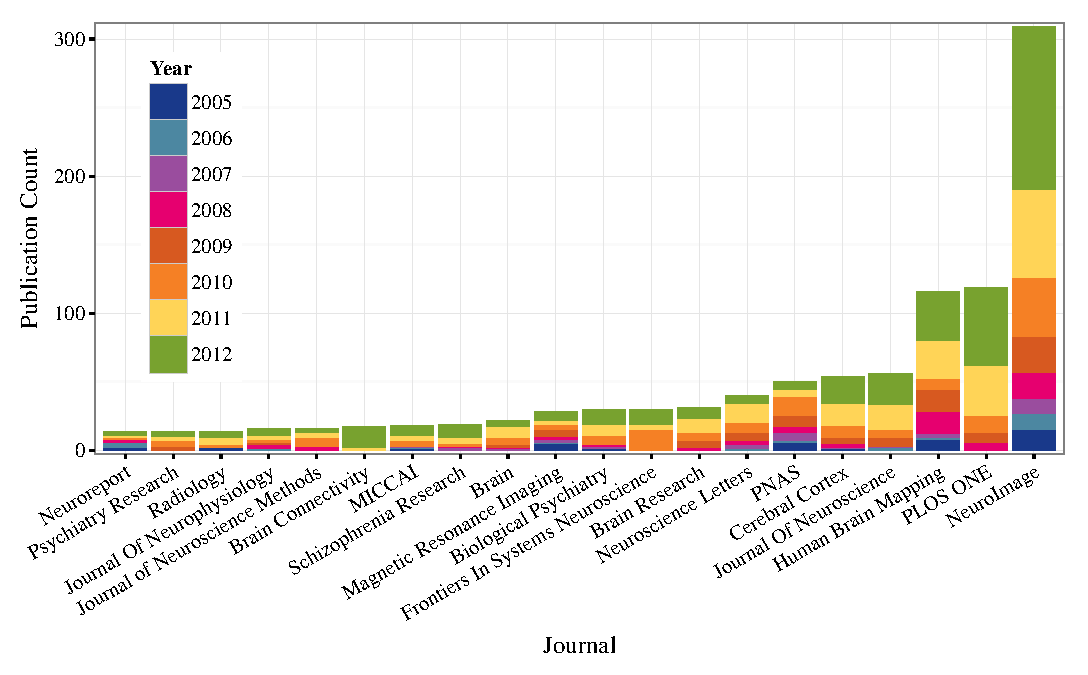
\includegraphics[]{figures/journal_dist}%
    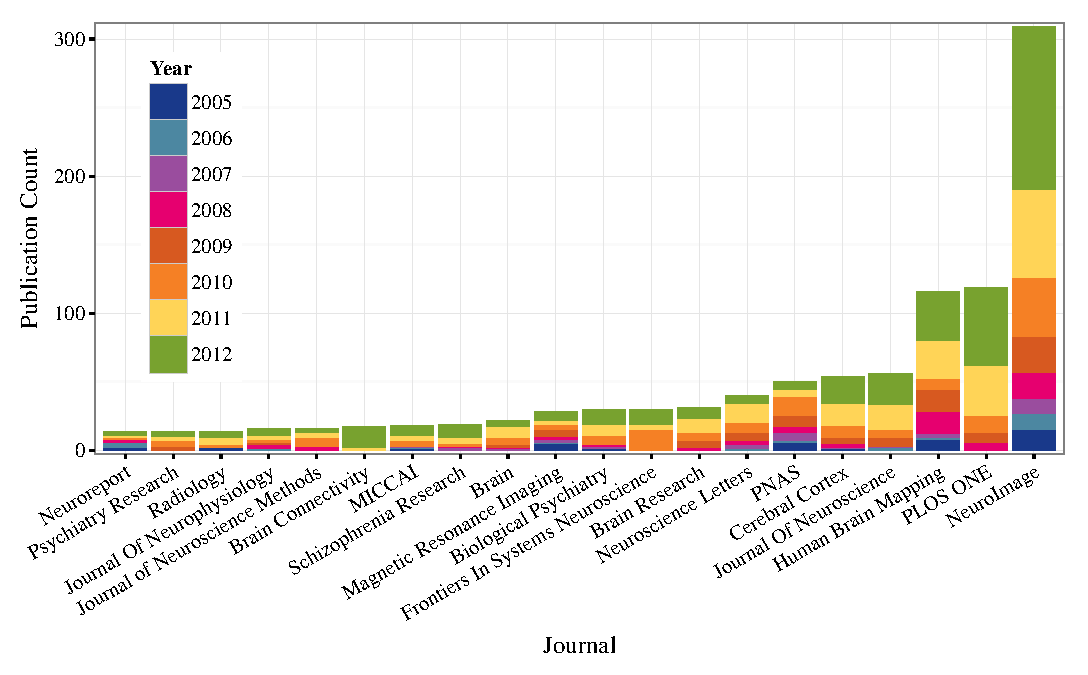
\includegraphics[]{figures/journal_dist}%
    %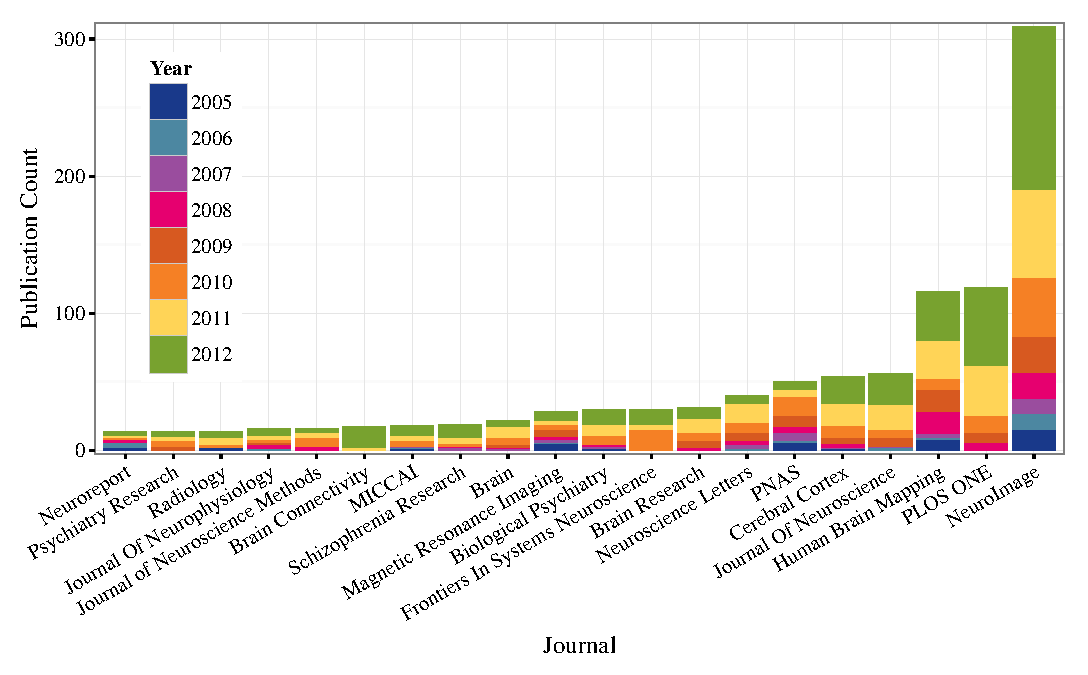
\includegraphics[width=\linewidth]{figures/journal_dist}%
    %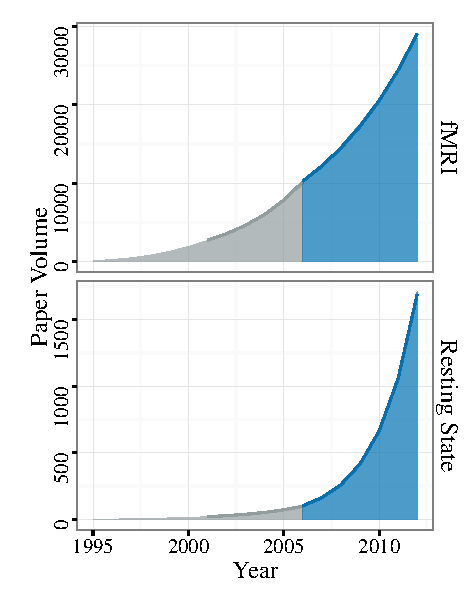
\includegraphics[width=.5\linewidth]{figures/overall_growth}%
    \caption{Publication counts by journal.
        \label{fig:journal_dist}
    }
  \end{center}
\end{figure*}

The density-equalizing map is shown in Fig.
\ref{fig:resting_state_map}.  The top three countries are the United States of
America, United Kingdom, and Netherlands, wherein lie 62.9\%, 9.6\%, and 8.6\%
of correspondence addresses, respectively.
\COMMENTCC{Re-color the density map so that the colors are meaningful, and are
more attractive.} 

%{{{------ Figure 3 -----}}}
\begin{figure}
  \begin{center}
    %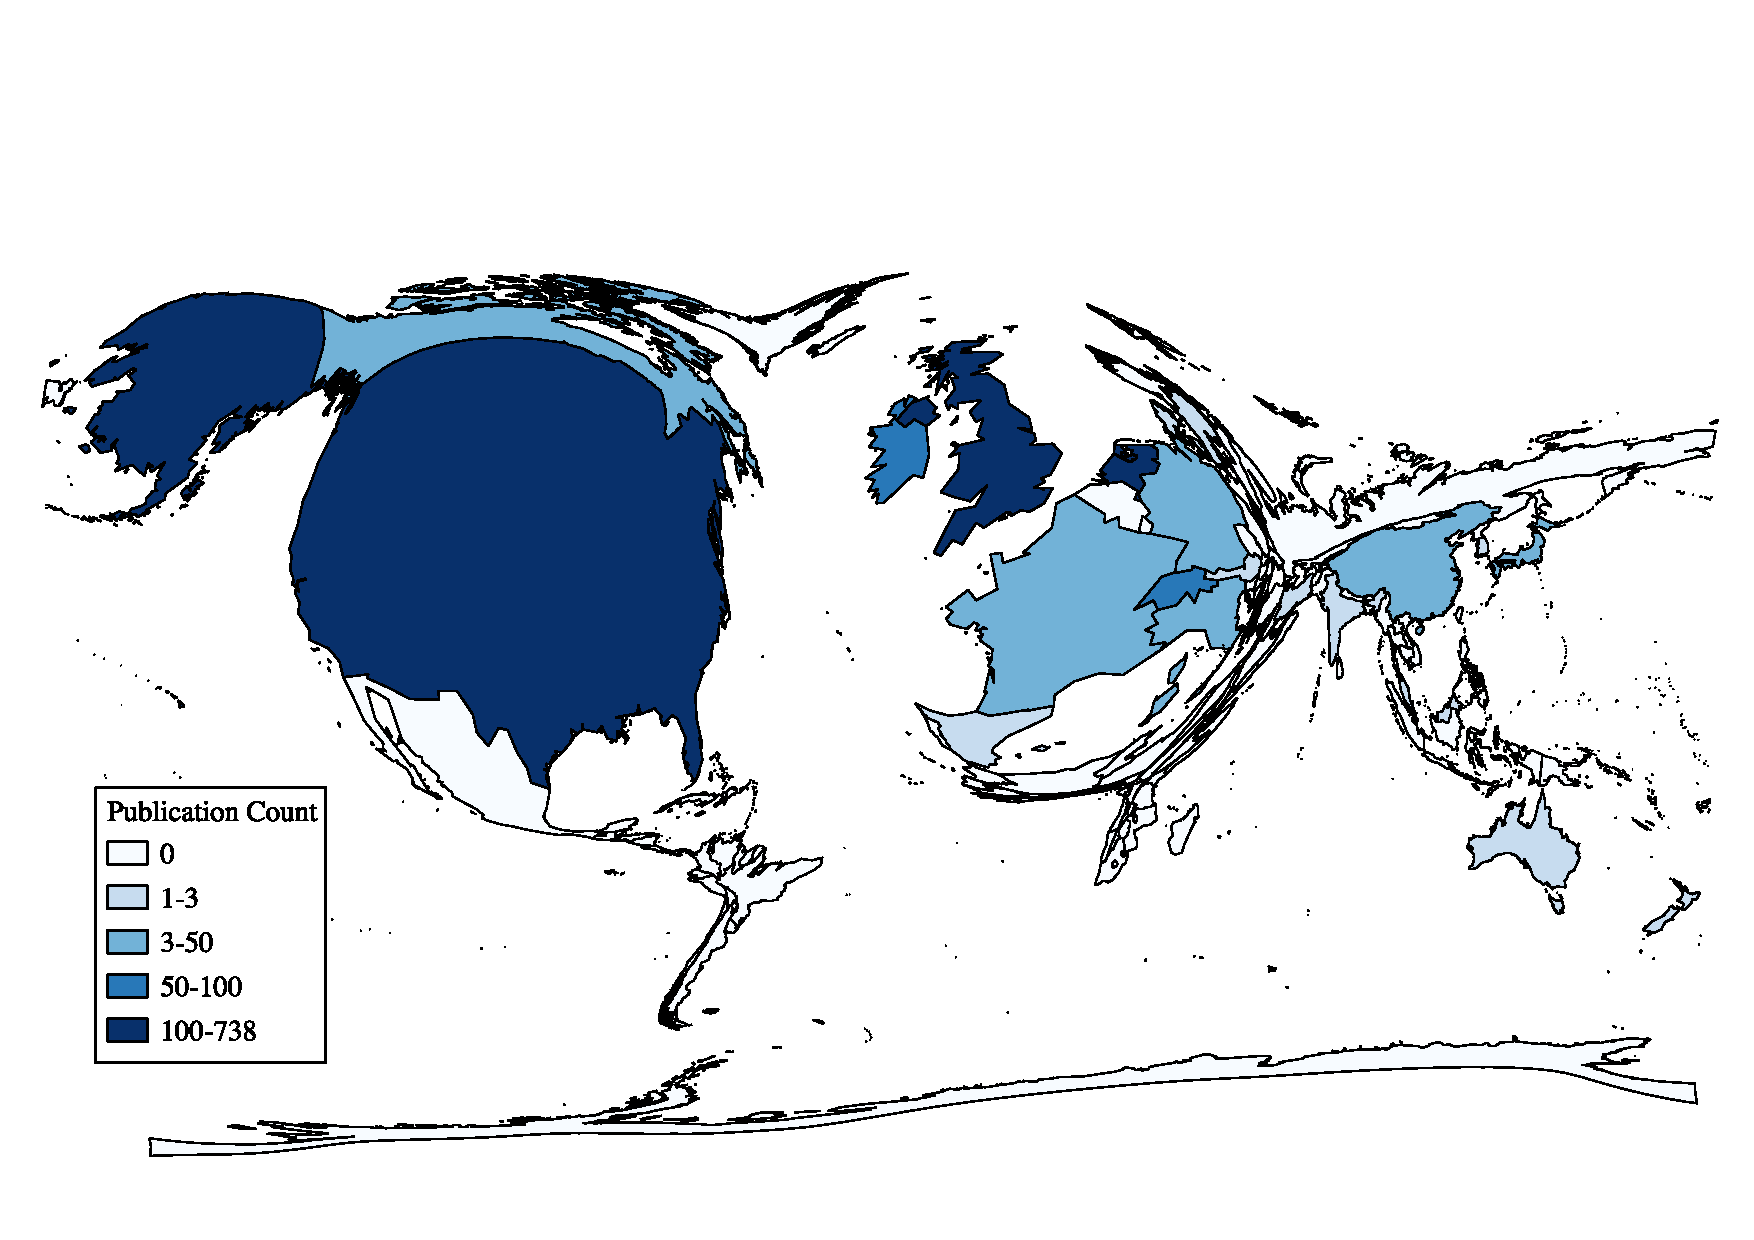
\includegraphics[]{figures/resting_state_map}%
    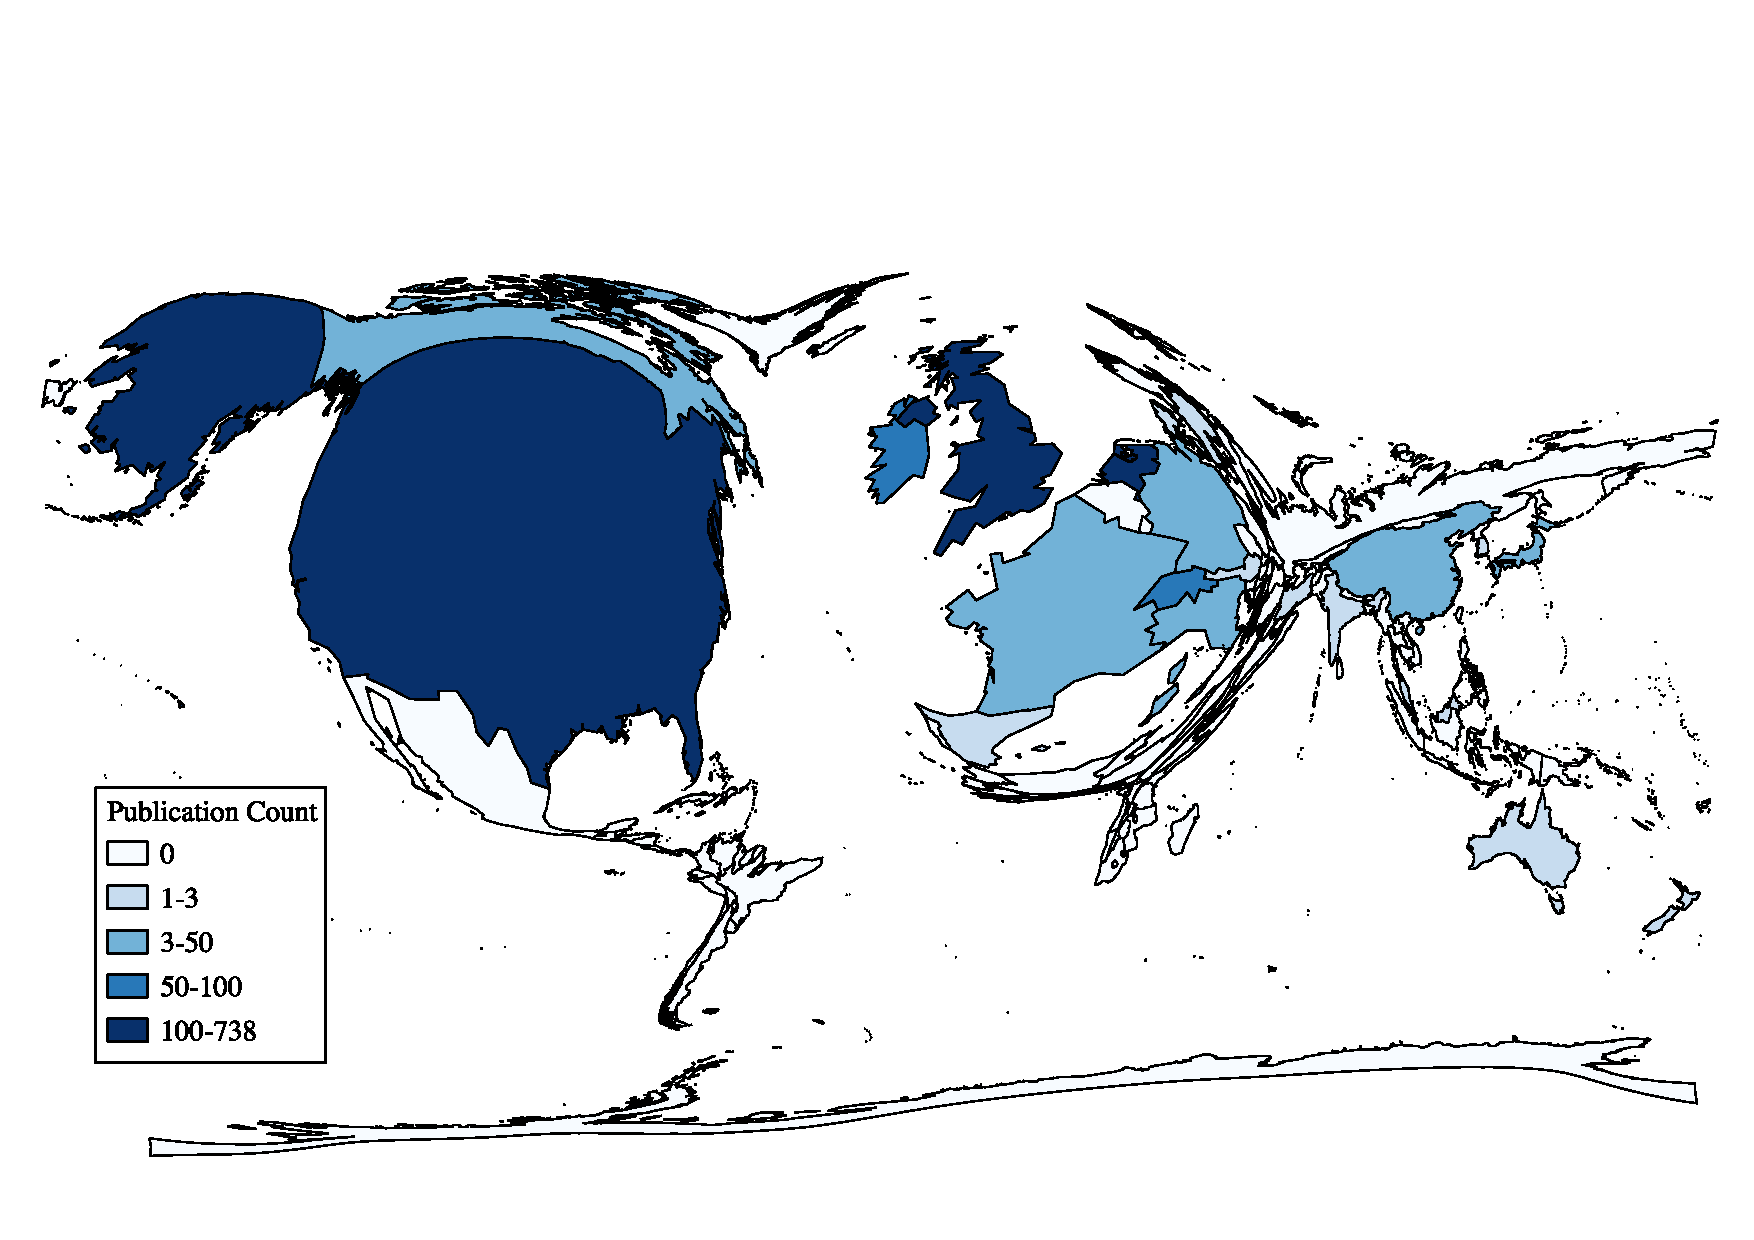
\includegraphics[width=\linewidth]{figures/resting_state_map}%
    %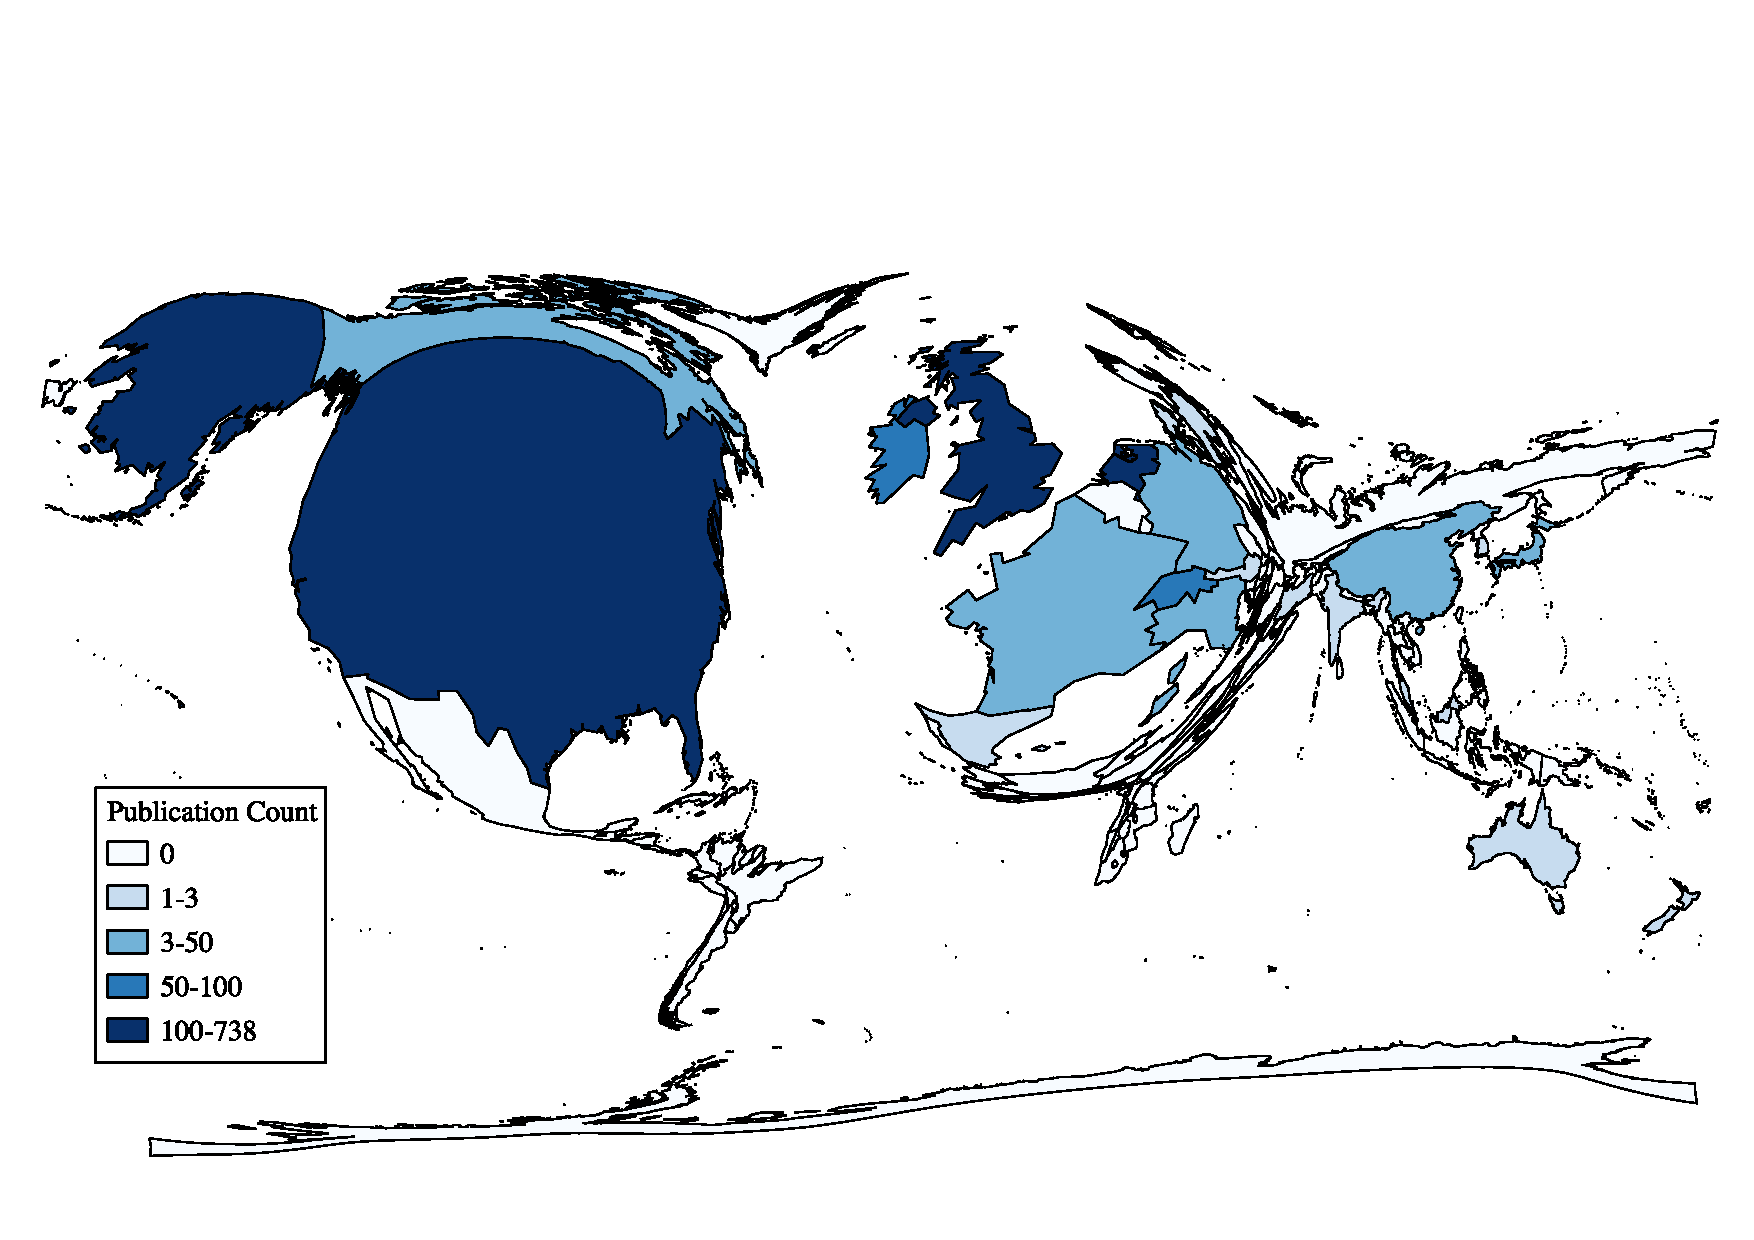
\includegraphics[width=.5\linewidth]{figures/resting_state_map}%
    \caption{Amount of resting state publications by country.
        \label{fig:resting_state_map}
    }
  \end{center}
\end{figure}


\subsection{Term Frequency Analysis}

\begin{table}[H]
\caption{\label{tagfreqtable} The number and fraction of publications in the
library tagged with a specific keyword}
\begin{center}
\begin{tabular}{|l|r|}
\hline
{\bf CMI Librarian Tag}&{\bf Frequency} \\ \hline \hline
Clinical & 747 (43\%) \\ \hline
Basic Neuroscience&593 (34\%) \\ \hline
Meta-analysis/reviews&235 (14\%) \\ \hline
Methodology&210 (12\%) \\ \hline
Multimodal&143 (8\%) \\ \hline
Brain and Behavior&79 (5\%) \\ \hline
1000 Functional Connectomes&61 (4\%) \\ \hline
Animal Models&61 (4\%) \\ \hline
Functional Anatomy&44 (3\%) \\ \hline
Genetics&29 (2\%) \\ \hline
\end{tabular}
\end{center}
\end{table}


Growth of the most prevalent clinical terms is shown in Fig.
\ref{fig:clinical_bytag_hist}. Of 1,721 publications in the corpus,
``Clinical'' is the most commonly applied tag (Tab. \ref{tagfreqtable}).
``Schizophrenia'' (13\%), ``Alzheimer's Disease'' (11.3\%), and
``Depression'' (10.8\%) are the most common clinical sub-tags that
co-occur with the ``clinical'' tag.

%{{{------ Figure 4 -----}}}
\begin{figure*}
  \begin{center}
    %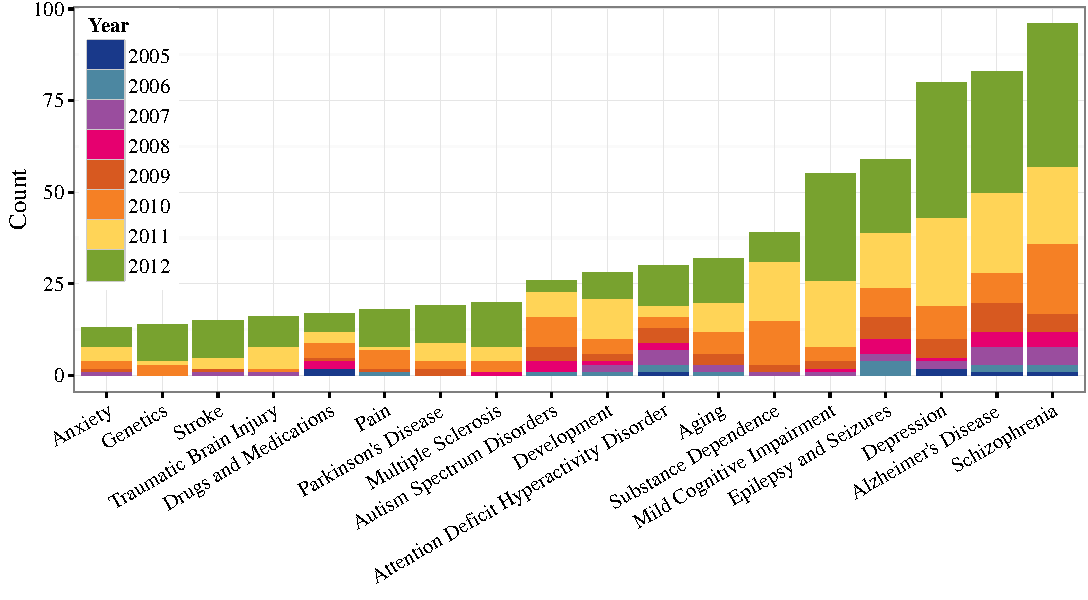
\includegraphics[]{figures/clinical_bytag_hist}%
    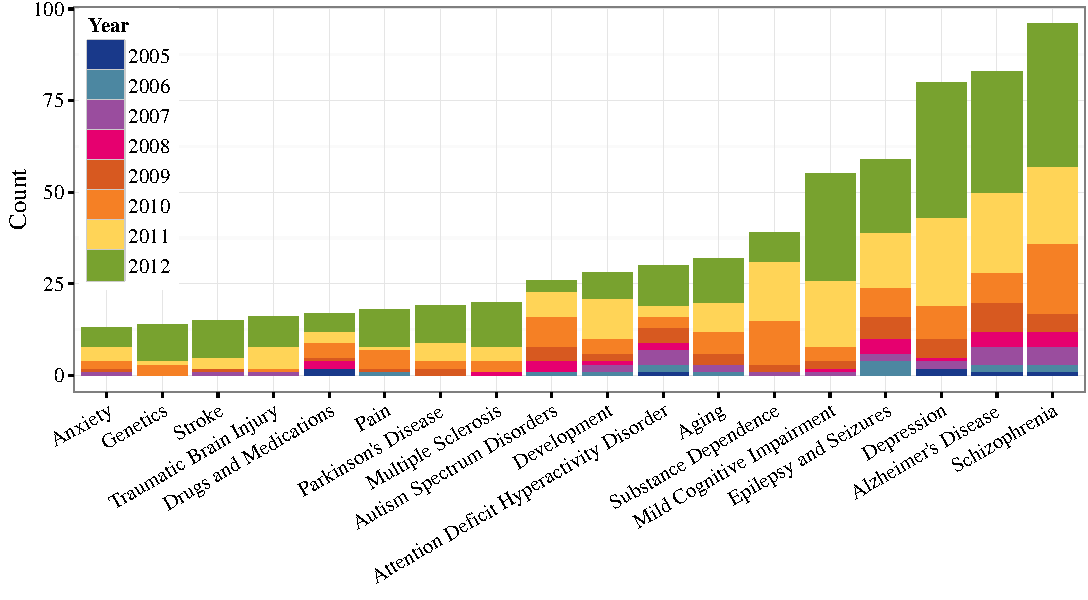
\includegraphics[]{figures/clinical_bytag_hist}%
    %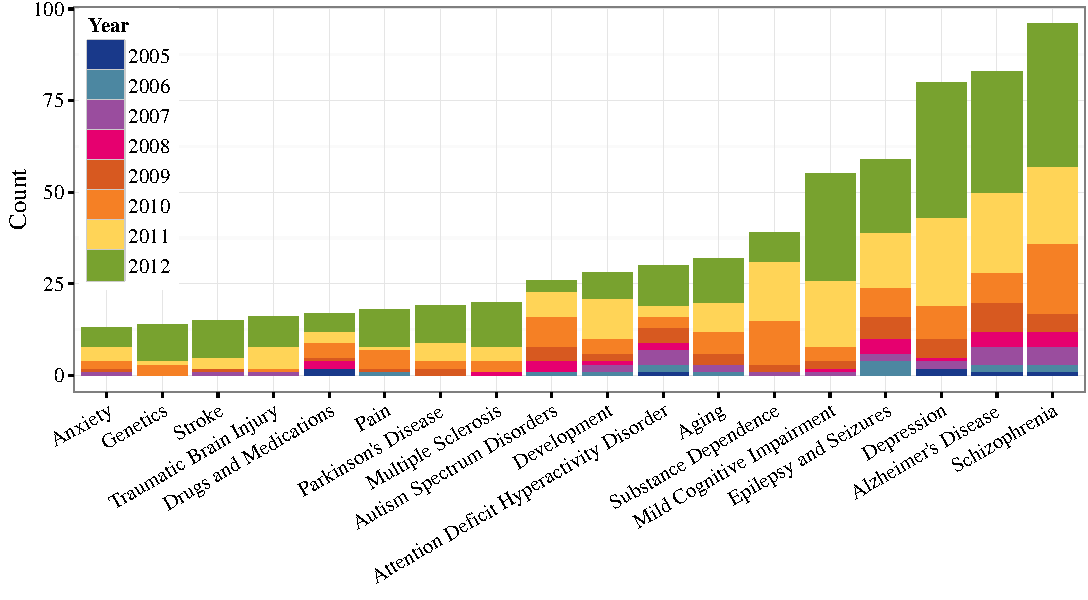
\includegraphics[width=.5\linewidth]{figures/clinical_bytag_hist}%
    \caption{Most common clinical terms from the resting state literature.
        \label{fig:clinical_bytag_hist}
    }
  \end{center}
\end{figure*}

Fig. \ref{fig:connectome_growth} shows growth of the term ``connectome'' in the
corpus. \COMMENTCC{Rather than using the plot for connectome growth, just
	mention the numbers in the text.} Term frequency ($t\!f$), document
frequency ($d\!f$), and term frequency-inverse document frequency ($t\!f \times
d\!f^{-1}$) have all increased since 2009.  

%{{{------ Figure 5 -----}}}
\begin{figure}
  \begin{center}
    %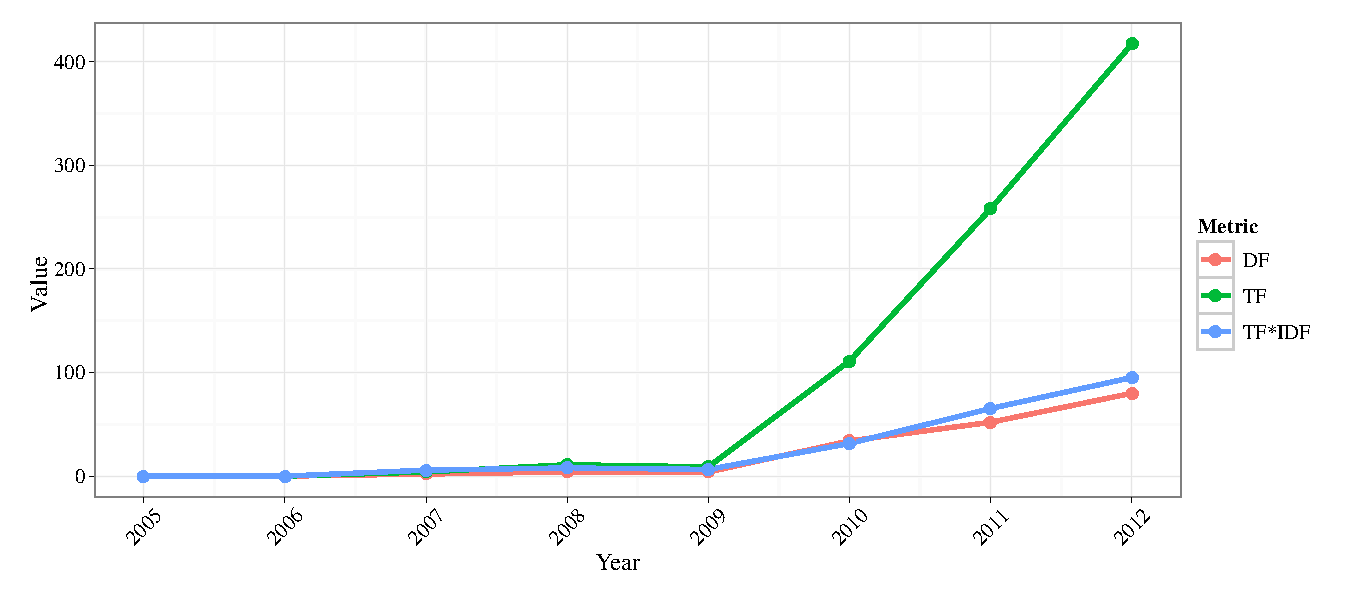
\includegraphics[]{figures/connectome_growth}%
    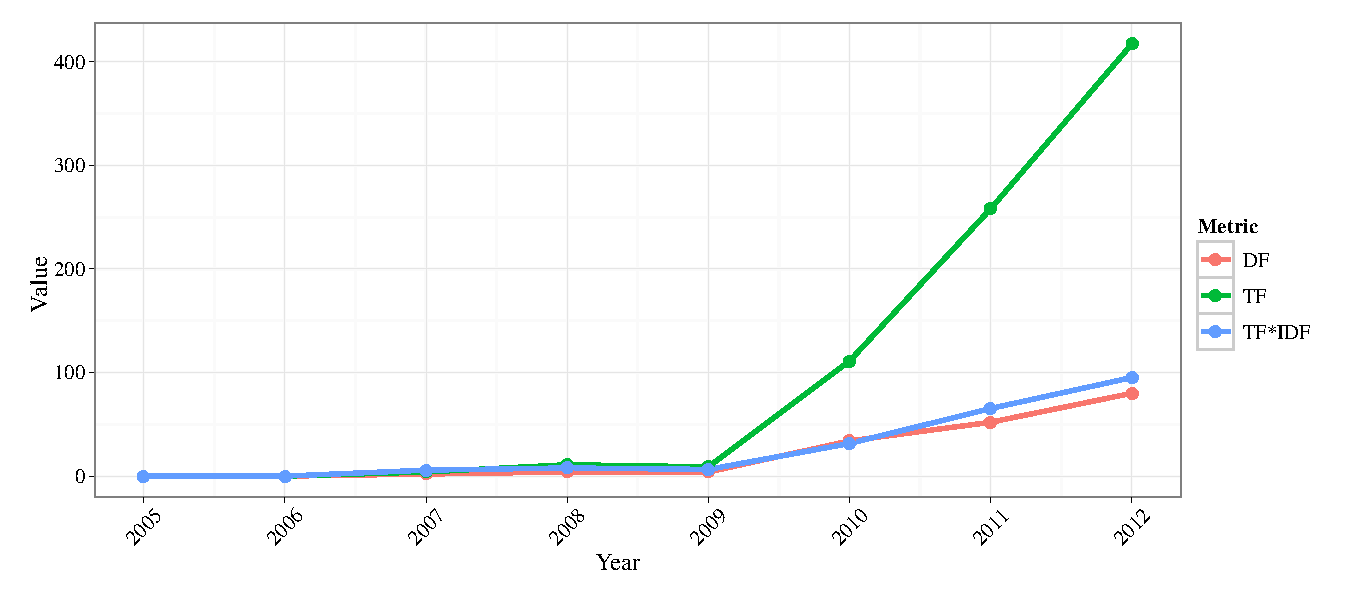
\includegraphics[width=\linewidth]{figures/connectome_growth}%
    %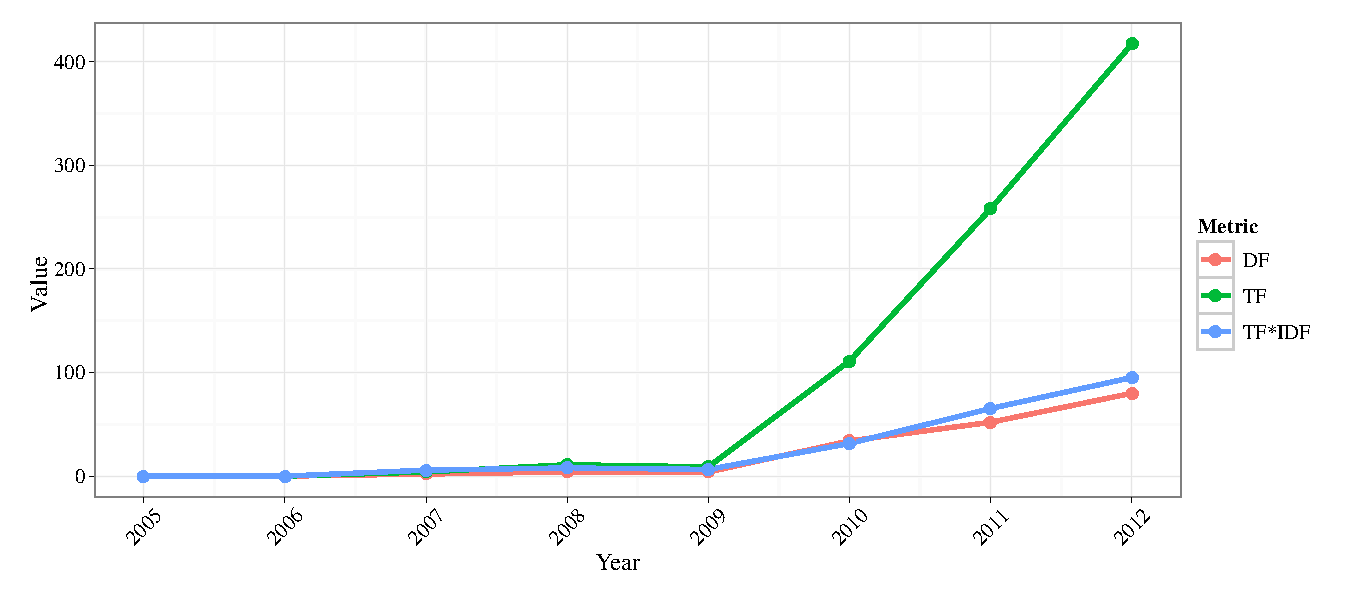
\includegraphics[width=.5\linewidth]{figures/connectome_growth}%
    \caption{Growth of use of term ``connectome'' in the corpus
        \label{fig:connectome_growth}
    }
  \end{center}
\end{figure}

Fig. \ref{fig:tfidf_top} shows conditional-$t\!f$ and $d\!f$ for the
terms with the highest values. The most common imaging modality was fMRI,
which was a key term in the searches used to generate the corpus. The most
investigated cognitive domains were activation, memory, attention, and
association. The PFC, PCC, and anterior cingulate were the most discussed
brain regions. 

%{{{------ Figure 6 -----}}}
\begin{figure*}
  \begin{center}
    %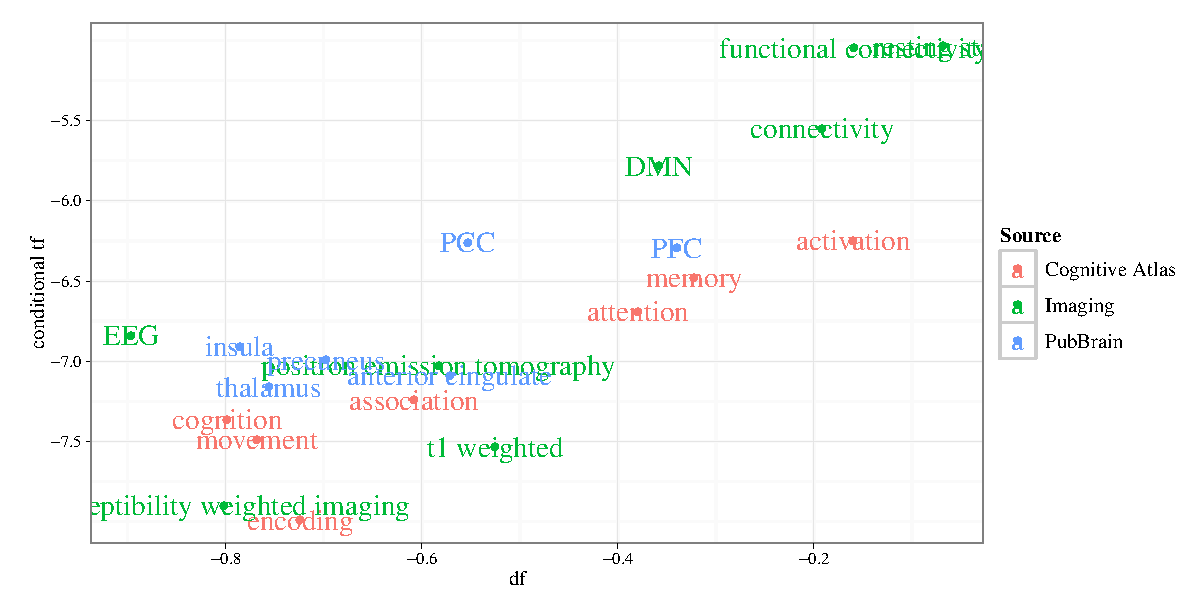
\includegraphics[]{figures/tfidf_top2}%
    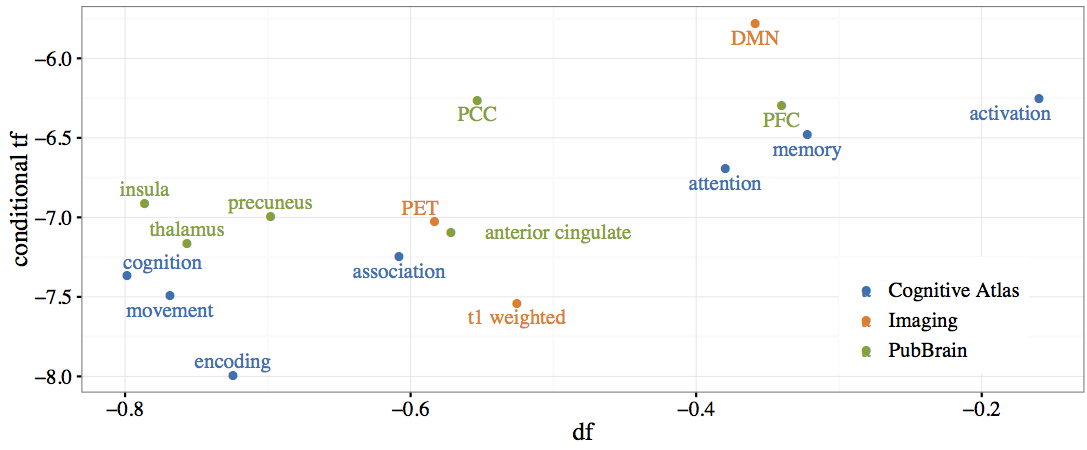
\includegraphics[]{figures/tfidf_top}%
    %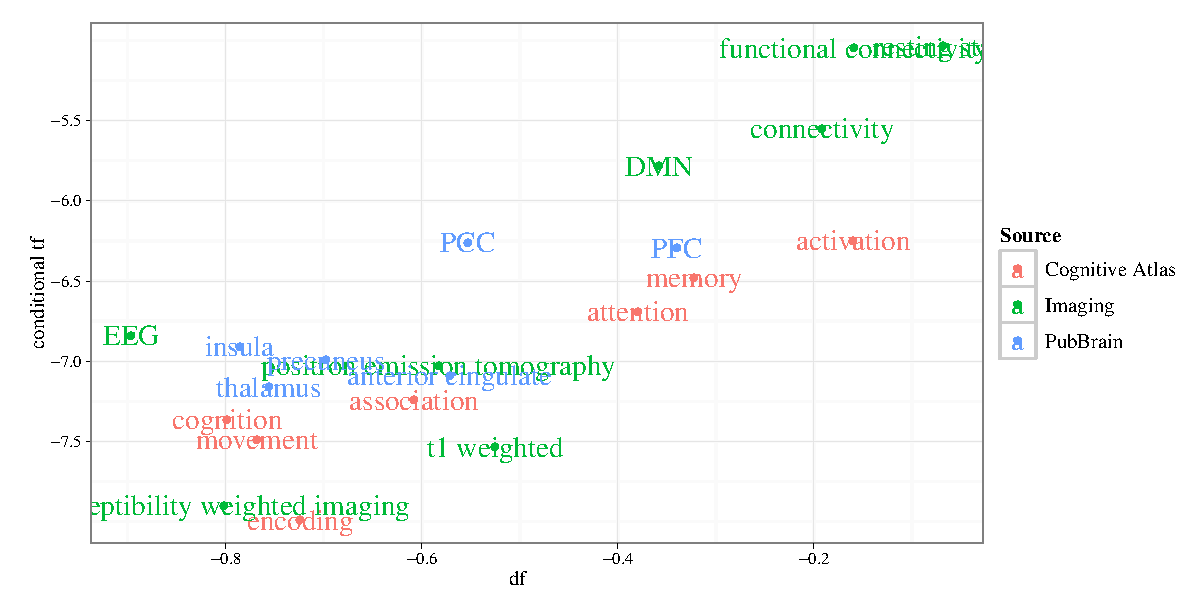
\includegraphics[width=.5\linewidth]{figures/tfidf_top2}%
    \caption{TF and conditional-DF for terms with the greatest values of each
    \label{fig:tfidf_top}
    }
  \end{center}
\end{figure*}

\subsection{Methods Analysis}

The accuracy of the Na\"ive Bayes model in inferring
algorithmic methods is shown in ??. \COMMENTCC{Table missing}

The terms used as features, along with their $\chi^2$ values, are shown in
??. \COMMENTCC{Table missing}

Fig. \ref{fig:methods_growth_hist} shows growth over time of algorithmic
methods in R-fMRI literature.  Seed-based correlation is by far the most
common method, accounting for nearly half of all uses of algorithmic
methods. Independent component analysis (ICA) and clustering have shown
steady growth since 2010, and use of machine learning methods increased at
a faster pace in 2012.

%{{{------ Figure 7 -----}}}
\begin{figure}
  \begin{center}
    %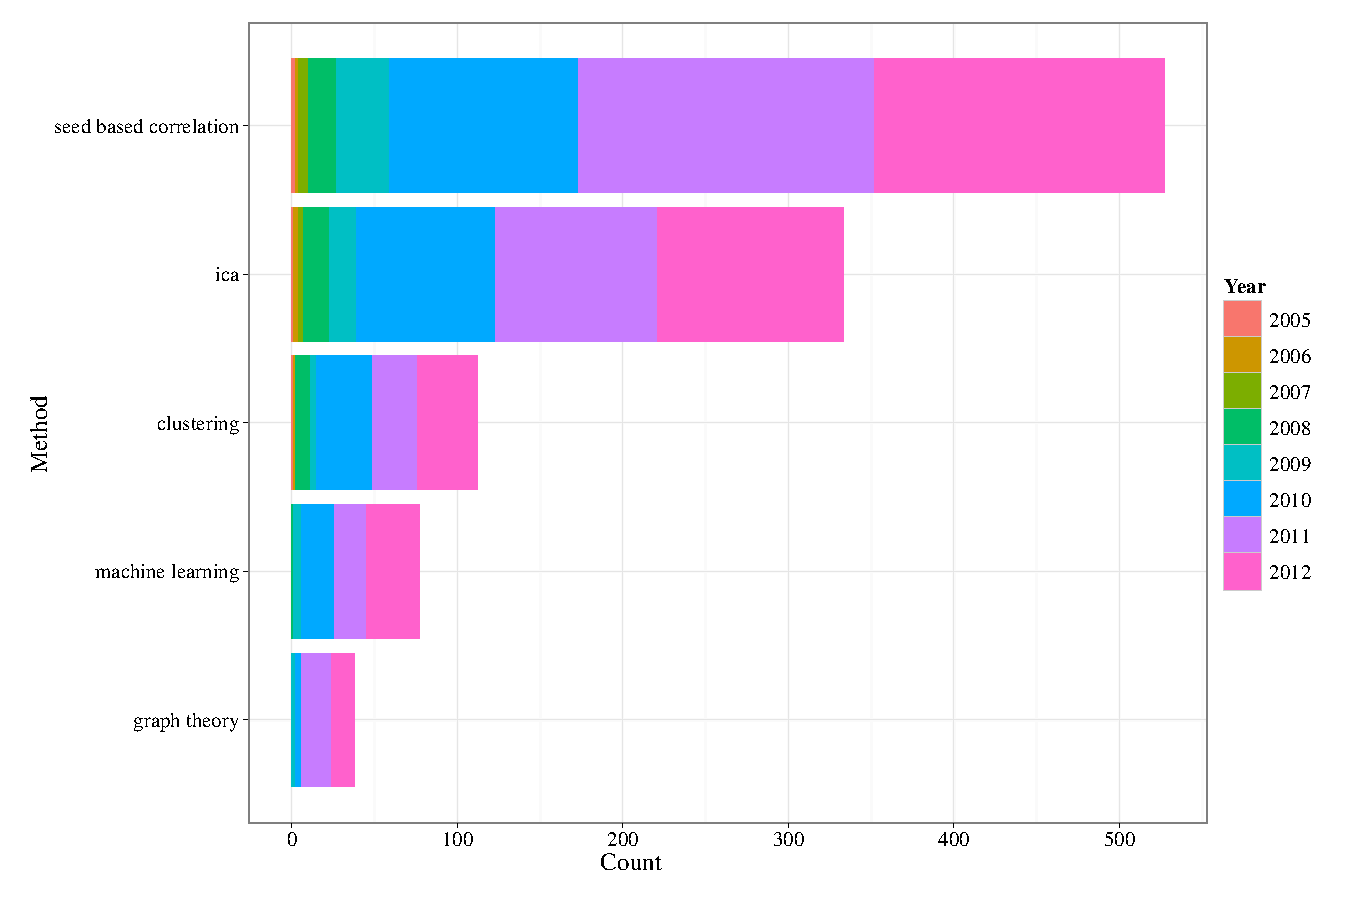
\includegraphics[]{figures/methods_growth_hist}%
    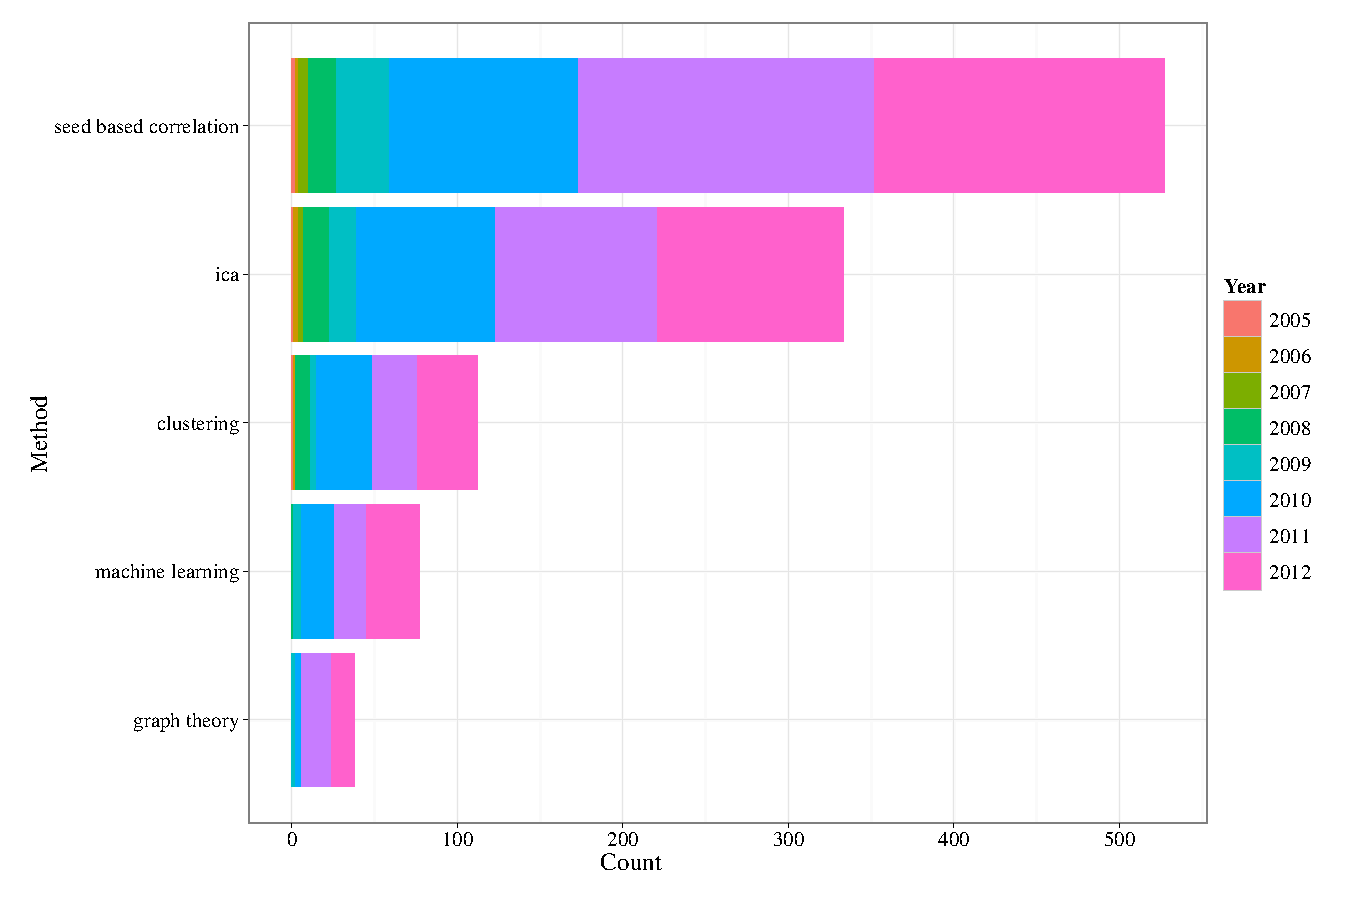
\includegraphics[]{figures/methods_growth_hist}%
    %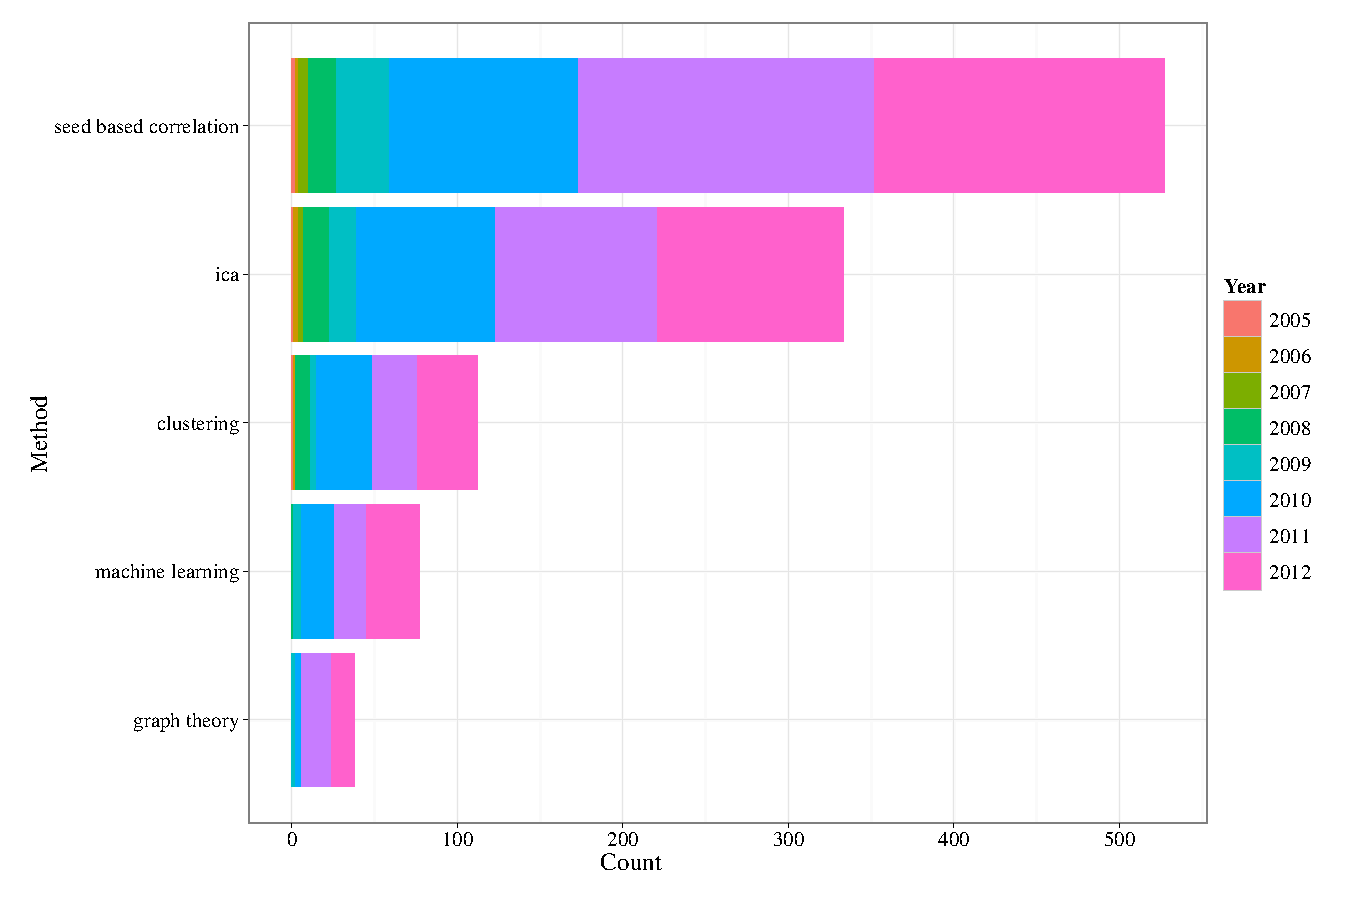
\includegraphics[width=.5\linewidth]{figures/methods_growth_hist}%
    \caption{Prevalence and growth of different methods applied in the resting
    state fMRI literature. 
        \label{fig:methods_growth_hist}
    }
  \end{center}
\end{figure}

%{{{------ Figure 8 -----}}}
\begin{figure}
  \begin{center}
    %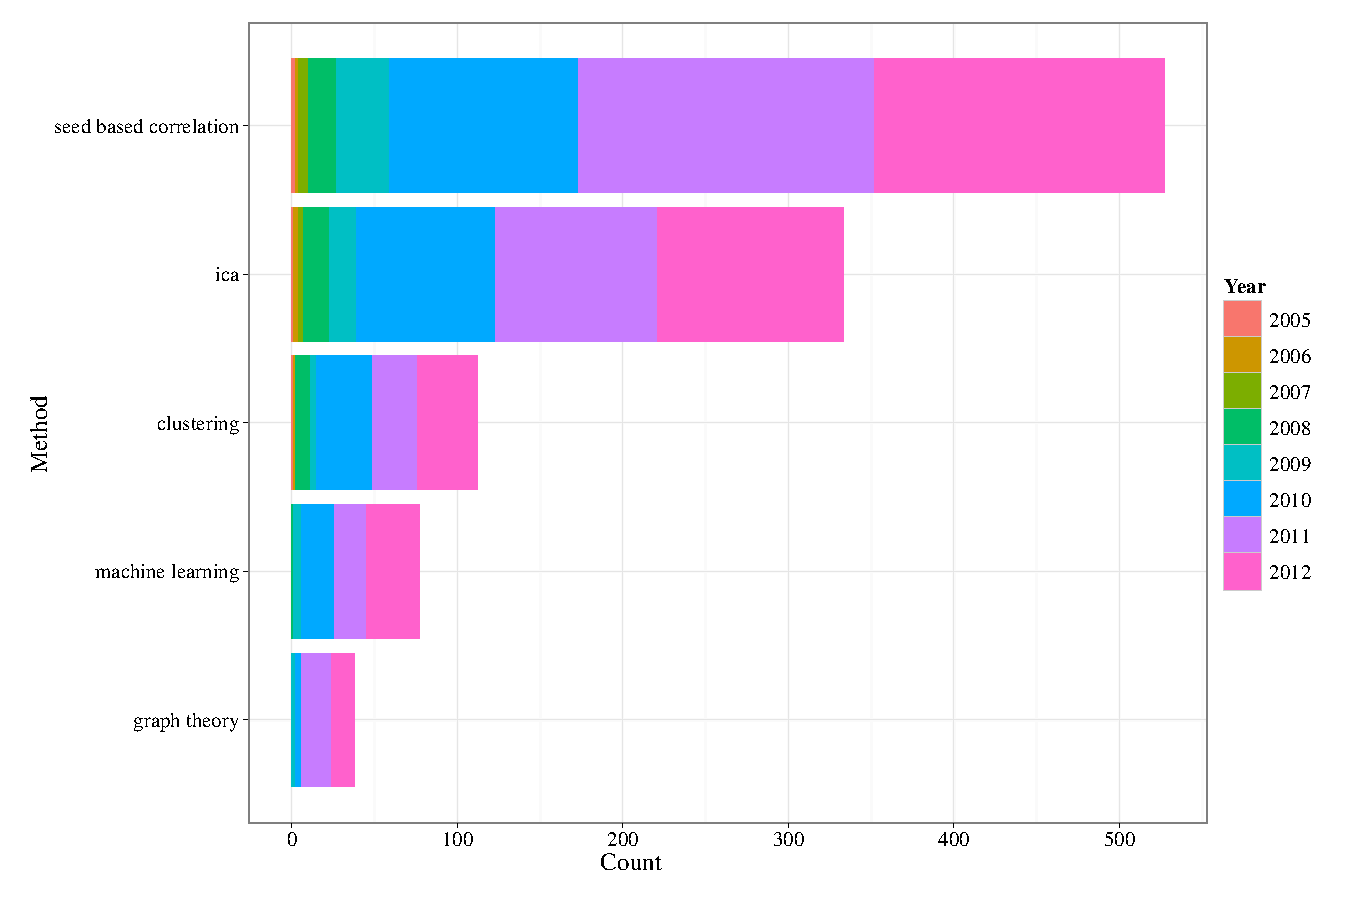
\includegraphics[]{figures/methods_growth_hist}%
    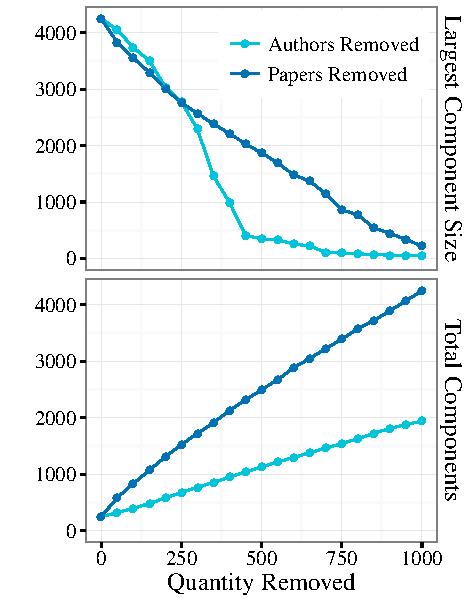
\includegraphics[]{figures/connected_after_removing}%
    %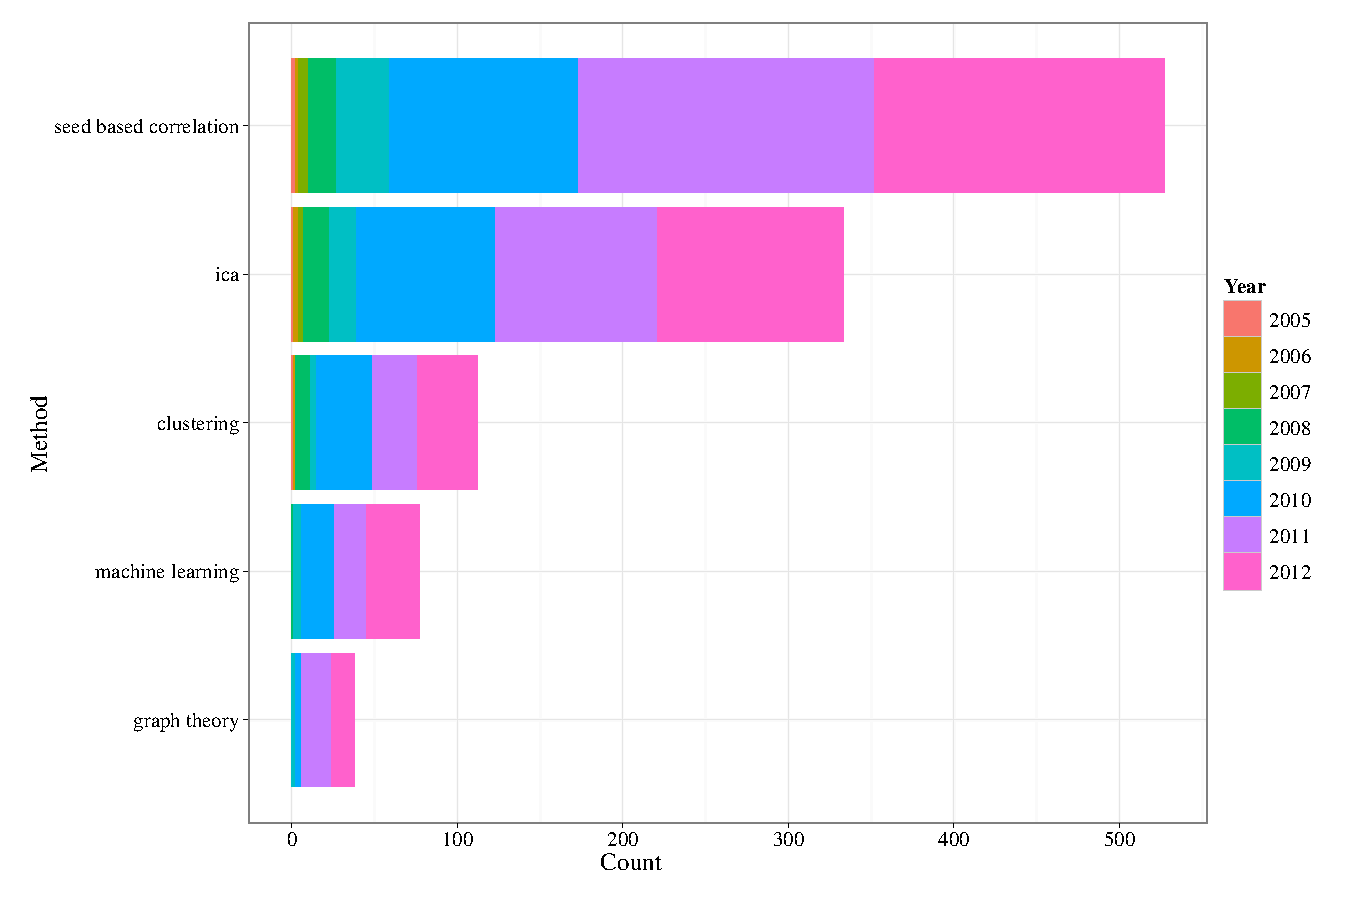
\includegraphics[width=.5\linewidth]{figures/methods_growth_hist}%
    \caption{Number of components and size of largest component after removing authors and papers from co-authorship graph.
        \label{fig:connected_after_removing}
    }
  \end{center}
\end{figure}

\subsection{Citation Analysis} 

\begin{table*}
	\caption{Publication Pageranks\label{table:pub_pageranks} }
%\begin{center}         % 7.25 inches
	\begin{tabular}{|m{.15in}|m{4.3in}|m{.3in}|m{1.1in}|m{.65in}|} \hline
		\# & Title & Year & Pagerank (SD) & Citations \\ \hline \hline 
		%\textbf{\#} & \textbf{Title} & \textbf{Year} &
		%\textbf{Pagerank (SD)} & \textbf{Citations} \\ \hline \hline 
		1 & A default mode of brain
		function.\cite{Raichle2001}&2001&0.0165 ($3\cdot\!
		10^{-4}$) & \textcolor{red}{MISSING}\\ \hline 
		2 & Functional connectivity in the motor cortex of resting
		human brain using echo-planar MRI.\cite{Biswal1995}&1995&0.0136
		($3\cdot\! 10^{-4}$) & \textcolor{red}{MISSING}\\ \hline
		3 & Functional connectivity in the resting brain: a network
		analysis of the default mode
		hypothesis.\cite{Greicius2003}&2003&0.0104 ($2\cdot\!
		10^{-4}$)& \textcolor{red}{MISSING}\\  \hline
		4 & Consistent resting-state networks across
		healthy subjects.\cite{Damoiseaux2006}&2006&0.0098 ($2\cdot\!
		10^{-4}$)& \textcolor{red}{MISSING}\\  \hline
		5 & Investigations into resting-state
		connectivity using independent component
		analysis.\cite{Beckmann2005}&2005&0.0069 ($2\cdot\!
		10^{-4}$)& \textcolor{red}{MISSING}\\  \hline
		6 & Functional connectivity in single and
		multislice echoplanar imaging using resting-state
		fluctuations.\cite{Lowe1998}&1998&0.0056 ($2\cdot\! 10^{-4}$)
		& \textcolor{red}{MISSING}\\  \hline
		7&Default-mode network activity distinguishes Alzheimer's
		disease from healthy aging: evidence from functional
		MRI.\cite{Greicius2004}&2004&0.0056 ($2\cdot\! 10^{-4}$)
		& \textcolor{red}{MISSING}\\ \hline
		8&Toward discovery science of human brain
		function.\cite{Biswal2010}&2010&0.0055 ($2\cdot\! 10^{-4}$)
		& \textcolor{red}{MISSING}\\  \hline
		9&Dissociable intrinsic connectivity networks for salience
		processing and executive control.\cite{Seeley2007}&2007&0.0055
		($10^{-4}$) & \textcolor{red}{MISSING}\\  \hline
		10&Intrinsic functional architecture in the
		anaesthetized monkey brain.\cite{Vincent2007}&2007&0.0047
		($10^{-4}$) & \textcolor{red}{MISSING}\\  \hline
\end{tabular}
%\end{center}
\end{table*}

\COMMENTCC{I think that the citation analysis  works better as a table
	(\ref{table:pub_pageranks}) than a graph. We have space to add the next
	10 papers, and the citation counts. also add in gephi plot of citation
	network} 

The top 10 publications by pagerank were collectively cited by 66\% of the
corpus, and the top 1\% of publications account for 10\% of the total
pagerank.  After these publications, pagerank falls off more slowly, with
the next 10\% of publications accounting for 40\% of the total pagerank. 

The mean clustering coefficient was 0.094 (standard error 0.010) and the
mean shortest path length was 4.4 (standard error 0.080). In a set of
1,000 random graphs constructed on the same set of vertices, the mean
clustering coefficient was 0.014 (standard error 0.0030) and the mean
shortest path length was 4.1 (standard error (0.60).

\subsection{Co-authorship Analysis} The co-authorship graph was found to
be robust, exhibiting significant small-world statistics. In particular,
its clustering coefficient was 0.878, compared to 0.002 for a random graph
with the same number of nodes and edges, and its average shortest path
length was 4.964, compared to 3.915 for the random graph.

Fig. \ref{fig:connected_after_removing} shows the number of connected components, and
size of the largest connected component, as publications and authors are
removed.  

\subsection{Working Groups Analysis}
Four working groups were identified. Their combined 23 authors (0.6\% of
3,704 across the literature) cover 17.5\% of R-fMRI publications. The mean
publication count by authors in these groups was 21.9; overall, it was
0.31. The mean number of publications in common between pairs of authors
in the same working group was 10.7; across different working groups, it
was 0.11.  

Working group authors (number of publications in corpus by author):
\begin{enumerate}
\item Michael P. Milham (41), F. Xavier Castellanos (37), Bharat Biswal
(36), and Clare Kelly (36)
\item Tianzi Jiang (35), Kun-Cheng Li (27), Chunshui Yu (19), Li-Xia Tian
(18), Yong Liu (15), and Yuan Zhou (15)
\item Qi-Yong Gong (35), Yi-Jun Liu (21), Hua-fu Chen (20), Wei Liao (20),
Guang-Ming Lu (18), Zhiqiang Zhang (17), and Yuan Zhong (13) 
\item Bradley L. Schlaggar (19), Steven E. Petersen (16), Alexander L.
Cohen (13), Damien Fair (13), Nico U. F. Dosenbach (10) and Fran M. Miezin
(10)
\end{enumerate}

\section{Discussion}

Our bibliometric analysis of R-fMRI literature lends insight into the
current state of the field, demonstrating its strength, areas of focus,
and future potential. The growth of R-fMRI literature is currently
significantly faster than fMRI, though R-fMRI currently comprises a small
fraction of the total volume of fMRI literature. A high rate of
publication growth likely indicates not only that researchers in the field
are publishing more, but also that the field is growing to include new
researchers.  The journal Neuroimage has published more R-fMRI literature
than any other. In general, nearly 50\% of the literature was published in
general neuroimaging journals, perhaps reflecting the rapid advancement of
methods used to study R-fMRI over the past 10 years. 

\COMMENTCC{Need a table with these counts.}

In contrast, only 1\% was published in clinical journals, suggesting that
the field has not yet matured enough to be used in clinical applications.
But despite their venues, a full 35\% of the R-fMRI corpus was tagged
“Clinical.” Indeed, a great proportion of R-fMRI research is performed on
both clinical and control populations in order to identify differences
between them; typically, however, the results of these experiments are not
immediately applicable in clinical medicine. \COMMENTCC{this is a odd
statement}

Another pattern that was explored, open access, is a relatively recent
innovation that allows researchers to access publications without payment
to the journal by either front-loading the cost onto the author or
subsidizing the cost in another way. Open access is not universal in
R-fMRI (26\%) or fMRI (22\%), but has strong footholds in both. That the
rate of open access is consistently increasing over time in both
literatures bodes well for the future of open science. \COMMENTCC{May want
to include information about the NIH mandate that publications resulting
from their grants be published open-access.}

Word frequency analysis easily identified the corpus domain, fMRI, as the
most common imaging modality. In addition, there was a focus on the
prefrontal cortex (PFC), which is implicated in executive function, as
well as on the posterior cingulate cortex (PCC), which is a central node
of the DMN \COMMENTCC{citation here}.  Notably, neither the parietal
cortex nor any of its subregions appear in the top hits, though they are
also implicated in the DMN. This result may demonstrate the bag of words
model’s limited ability to aggregate concepts: for example, it may be the
case that the sum of occurrences of subregions of the parietal cortex
would appear in the top hits, but none appear individually. Finally,
memory and activation were the most discussed cognitive domains,
reflecting current research trends such as in \COMMENTCC{missing citation
[8]} and \COMMENTCC{missing citation [9]}. A possible extension of this
research is to identify common terms across scientific fields to
determine, for example, whether particular genes can affect PFC and PCC
function \COMMENTCC{this is not clear}.

Analysis of working groups found particularly prolific labs and
collaborators, offers measures for whether the field is dominated by only
a few authors, and found patterns in geographic localities and language.
The resulting groups are together responsible for nearly a fifth of the
total corpus, including some of the highest-Pageranked publications,
though there is little publication overlap between groups. Ranking authors
by their impact factor reveals that several of the authors in these
groups, including M. P. Milham, F. X. Castellanos, C.  Kelly, B. Biswal,
and Qi-Yong Gong, are not only prolific, but also are attributed many
citations. Furthermore, geographic location, language, and affiliation are
consistent within groups, but very different between groups: M. P.
Milham’s group is based in New York, T. Z. Jiang’s group is based in
Beijing, Qi-Yong Gong’s group is based in Sichuan, and Bradley Schlaggar’s
group is based in St. Louis.  This result demonstrates the strength of
R-fMRI research around the world, and suggests that distance, time zone,
and language pose practical barriers to collaboration \COMMENTCC{this
statement is pushing it}.

Analysis of the citation graph concluded that it can be considered ``small
world'' because its mean clustering coefficient is significantly higher
than that of a random graph, and its mean shortest path length is not
significantly different from that of a random graph \cite{Watts1998}. In a
small world network, most nodes are not adjacent to one another, but the
mean path length is still fairly short because there are few degrees of
separation needed to reach one node from another. More precisely, the mean
path length of a small world network grows with the logarithm of the total
number of nodes. In this application, this result indicates that although
most publications do not cite a large fraction of the corpus, but the
number of hops needed to traverse from one publication to another is still
fairly short. \COMMENTCC{What qualifies as a large fraction here? We
should offer something better to back up this statement} Indeed, there are
many real-world relationships, such as social networks and Internet
connections, that can be represented with small world graphs. 

By measuring Pagerank, publications were identified that are central to
R-fMRI literature without necessarily having the highest raw citation
count. Among the highest Pageranked publications are the seminal
publications that provide much of the historical groundwork for the field.
Indeed, from these publication emerges a narrative of R-fMRI history, from
the foundations of R-fMRI functional connectivity and activation, to the
first clinical application in the field, to the discovery of the canonical
independent R-fMRI networks.  Relatively consistent Pageranks among the
remaining publications suggest that the field is not completely
represented in only a small subset of the corpus, but rather is still
growing in high-impact directions. 

The publication with the second highest Pagerank, Biswal et al’s
``Functional connectivity in the motor cortex of resting human brain using
echo-planar MRI'' (1995)\cite{Biswal1995}, demonstrated functional
connectivity in spontaneous, low frequency activity measured using R-fMRI.
Resting state functional connectivity had been observed in clinical
settings for a long time using electroencephlogram (EEG), and positron
emission tomography (PET), which measures glucose metabolism. However,
this was the first time it was observed in the complex fMRI-measured BOLD
signal, which lacks clear physiological underpinning. Bharat Biswal
appears in a top working group and in the list of highest impact authors.
Functional connectivity, first demonstrated with R-fMRI in this
publication, is among the most frequently occurring terms in the corpus
\COMMENTCC{the corpus is determined by the presence of the term functional
connectivity}. 

Another, separate line of research took root with a series of 2001
publications that include those with first and seventh highest pagerank,
Raichle et al’s ``A default mode of brain function,'' and Gusnard et al’s
``Searching for a baseline: functional imaging and the resting human
brain.'' These publications established that decreases of brain activity
that occur during rest are spatially consistent, and introduced the notion
of a functional default mode. This line of research on activation was
cognitive neuroscience’s contribution to the foundations of R-fMRI theory.
Indeed, activation was found to be among the most frequent cognitive terms
in the corpus.

These disparate contributions from neuroimaging and cognitive science were
married in the third highest pageranked publication, Grecius et al’s
``Functional connectivity in the resting brain: a network analysis of the
default mode hypothesis'' (2003). Grecius showed that, in fact, the
regions that show correlation during rest are also activated during rest.
Thus, this publication introduced the notion of the default mode network,
whose regions show both low frequency correlation of spontaneous activity
during rest, and also decreased task-related activity. Notably, the
default mode network is among the most common neuroimaging terms in the
corpus.

In 2004, Grecius followed with the fifth highest pageranked publication,
''Default-mode network activity distinguishes Alzheimer’s disease from
healthy aging: evidence from functional MRI.'' This work linked clinical
neuroscience with R-fMRI functional connectivity by demonstrating with
fMRI not only that resting state activity was reduced in Alzheimer’s
patients, but also that the regions in which R-fMRI activity was reduced
were the very same that had been previously implicated in Alzheimer’s
disease. 

In 2006, DeLuca et al’s ``fMRI resting state networks define distinct
modes of long-distance interactions in the human brain'' found resting
state networks—regions that are individually correlated during rest—that
are independent both functionally and statistically. These networks have
been applied widely since their discovery, and appear in the list of most
common neuroimaging terms in the corpus.

\section{Conclusion}

Our bibliometric analysis demonstrates that, though still small compared
to fMRI, R-fMRI is a rapidly-growing field with major international
research hubs.  The research community is tight-knit, as shown by its
small world citation network, and the field is no one-trick pony, as shown
by the large number of highly-pageranked publications. The word frequency
analysis identified key concepts in use, and suggests future paths toward
integration of R-fMRI with other rapidly-growing fields such as genetics.

\section{Acknowledgements} This research was supported by the Child Mind
Institute Endeavor Scientist program.

{
%\clearpage
\section*{References}
%\small
\bibliographystyle{elsarticle-num-names}
\bibliography{rsbib_paper} 
}

\end{document}
